%% ch05_hni_onboarding.tex -- generated from fraud_detection_agent_interview_case_study.md
%% Do not edit by hand; edit the markdown and re-run build_tex.py.

\chapter{HNI Customer Onboarding Agent}
\label{chap:ch05_hni_onboarding}

% \section*{Chapter Purpose}
% \addcontentsline{toc}{section}{Chapter Purpose}
% \label{sec:ch05_hni_onboarding-chapter-purpose}

% This chapter presents a customer-onboarding fraud detection and KYC/EDD assessment system as a natural interview-style discussion. The interviewer begins with a vague problem statement. The candidate first discovers the business context, workflows, requirements, constraints, and success metrics. Only after confirming the scope does the candidate propose the architecture and implementation.

% The discussion is aligned with the implementation described in \texttt{NEW\_CASE\_STUDY.md}: a single FastAPI service, a production web UI with Document Upload, Name Search, and Historical KYC tabs, Postgres persistence, S3 or ADLS object storage, an in-memory document page index, deterministic UBO resolution, watchlist screening, risk scoring, OSINT enrichment, and LLM-generated EDD rationale.

% The central design principle is:

% \begin{quote}
% The LLM reads evidence and writes explanations. Python resolves ownership, matches watchlists, calculates risk, and decides the workflow outcome.
% \end{quote}
% The system supports two workflows:

% \begin{enumerate}[leftmargin=\speakwid]
% \item Document onboarding using uploaded KYC documents.
% \item Name-based OSINT search when documents are unavailable.
% \end{enumerate}
% Both workflows converge on the same deterministic ownership, screening, scoring, and EDD pipeline.

% \medskip\hrule\medskip
\section{Business Context and Stakeholders}
\label{sec:ch05_hni_onboarding-1-business-context-and-stakeholders}

\speaker{Interviewer}{I have a customer onboarding problem. We receive information about a client, and we want to decide whether the client is safe to onboard. Can you design a system for this?}

\speaker{Candidate}{Yes, I can. Before proposing a solution, can you brief me on the business context? Is this for bank-account onboarding, private banking, wealth management, payments, or something else? Also, what does ``safe to onboard'' mean in your process?}

\speaker{Interviewer}{This is for customer onboarding in a financial-services environment. The client may be an individual, company, trust, foundation, partnership, or holding structure. The operations team collects KYC documents and wants help identifying fraud, sanctions, politically exposed persons, adverse media, opaque ownership, and other risks.}

\speaker{Candidate}{That gives me a useful starting point. Is the system expected to make the final approval decision, or should it recommend an outcome for an analyst or MLRO to review?}

\speaker{Interviewer}{It should recommend an outcome. It must not replace the authorized compliance decision-maker.}

\speaker{Candidate}{Good. So this is a KYC and enhanced-due-diligence decision-support system, not an autonomous onboarding authority. The system can calculate a risk score, identify hard stops, recommend standard CDD, EDD, escalation, or decline, and produce an explanation. A human remains accountable for the final decision.}

\speaker{Interviewer}{Correct.}

\speaker{Candidate}{Can you explain where the current process is slow or unreliable?}

\speaker{Interviewer}{Analysts manually read application forms, trust deeds, ownership charts, IDs, and source-of-wealth documents. They identify the applicant and related parties, calculate beneficial ownership, check sanctions and PEP information, investigate public sources, assign a risk score, and write an EDD note. The process is slow, and the quality depends heavily on the analyst.}

\speaker{Candidate}{Understood. So the business problem is not only document extraction. It is a complete onboarding-risk workflow: understand the customer structure, identify UBOs, screen parties and jurisdictions, score risk, recommend the next compliance action, and explain why.}

\speaker{Interviewer}{Yes.}

\speaker{Candidate}{Does the system need to support a case where the client provides no documents but the analyst wants to search a name on public sources?}

\speaker{Interviewer}{Yes. There should be a Name Search workflow where the analyst provides a client name and optionally age or location. The system searches public information and creates a preliminary assessment.}

\speaker{Candidate}{Great. Then I see two related but different workflows: document-led onboarding and name-based OSINT screening. They should share the deterministic risk engine but have different evidence-collection steps.}

\subsection{Stakeholders}

\speaker{Candidate}{Before going further, I would list the stakeholders:}

\begin{enumerate}[leftmargin=\speakwid]
\item Customer-onboarding analysts, who submit documents or start a name search.
\item KYC operations teams, who verify identity and collect missing evidence.
\item Compliance officers and MLROs, who review escalations and suspicious findings.
\item Relationship managers, who need a clear explanation of onboarding blockers.
\item Financial-crime risk teams, who define watchlist and jurisdiction policies.
\item Legal and privacy teams, who govern handling of personal data and public information.
\item Engineering and platform teams, who operate the API, database, and storage.
\item Internal audit and regulators, who may request evidence of how a result was produced.
\end{enumerate}
\speaker{Interviewer}{Why include relationship managers if they do not make the compliance decision?}

\speaker{Candidate}{They often manage the customer relationship and respond to requests for missing documents. They need understandable explanations, but they should not be able to override screening or hard-stop rules without the appropriate compliance authority.}

\speaker{Candidate}{With stakeholders clear, can we lock the KYC requirements next --- inputs, UBO and screening outputs, and how we will measure success?}

\medskip\hrule\medskip
\section{Requirements and Success Metrics}
\label{sec:ch05_hni_onboarding-2-requirements-and-success-metrics}

\speaker{Interviewer}{Good. Now can you design the system?}

\speaker{Candidate}{I can, but before describing the solution, I want to clarify the exact requirements. I will start with the inputs and workflows, then discuss outputs, controls, and success metrics.}

\subsection{Functional Requirements Discovery}

\speaker{Candidate}{What information is mandatory for the document workflow?}

\speaker{Interviewer}{The user provides a client name, chooses \texttt{documents}, and uploads one or more PDF files. The files may include KYC application forms, trust deeds, ownership charts, incorporation certificates, identity documents, and source-of-wealth evidence.}

\speaker{Candidate}{Are the files required for the name-search workflow?}

\speaker{Interviewer}{No. For \texttt{name\_search}, the client name is enough. Age and location are optional in the web UI, although richer subject details can be provided through development interfaces.}

\speaker{Candidate}{Should the API accept scanned PDFs?}

\speaker{Interviewer}{Scanned documents are out of scope --- the design requires extractable text, provides no OCR, and fails a case when no usable text is extractable.}

\speaker{Candidate}{I would make that limitation visible to users. A silent ``no risk found'' result from a scanned document would be dangerous. The system should fail or mark the case as failed when it cannot extract usable text.}

\speaker{Interviewer}{Agreed.}

\speaker{Candidate}{What should the system extract from documents?}

\speaker{Interviewer}{Parties, party types, relationships, ownership edges, applicant metadata, source of wealth, and identity-verification details.}

\speaker{Candidate}{For ownership, do we need direct ownership only, or indirect ownership through multiple companies and trusts?}

\speaker{Interviewer}{Indirect ownership is important. The system should calculate effective ownership through chains and identify control roles such as settlor, trustee, protector, director, or signatory.}

\speaker{Candidate}{What threshold defines a beneficial owner?}

\speaker{Interviewer}{The default threshold is 25 percent, configurable through \texttt{UBO\_THRESHOLD\_PCT}.}

\speaker{Candidate}{What happens when ownership percentages are missing?}

\speaker{Interviewer}{The relationship may still provide control evidence, but the system should not invent an ownership percentage.}

\speaker{Candidate}{Good. The system can preserve the path as control evidence and use control roles independently from percentage ownership.}

\speaker{Candidate}{Which screening categories are required?}

\speaker{Interviewer}{Sanctions, PEP, adverse media, high-risk jurisdictions, and offshore indicators. Self-declared PEP status should also be considered.}

\speaker{Candidate}{Should my design call commercial sanctions or PEP databases?}

\speaker{Interviewer}{No. It uses sample reference lists or JSON-configured overrides. Name-search also uses web-derived evidence.}

\speaker{Candidate}{That distinction is important. I would not describe sample lists as production watchlist coverage. They are sample fixtures or configurable reference data.}

\subsection{Output Requirements}

\speaker{Candidate}{What should the assessment produce?}

\speaker{Interviewer}{It should produce UBOs, watchlist hits, geography hits, a risk score, a risk band, EDD triggers, a decision, a hard-stop reason if applicable, and an EDD rationale with recommended measures and missing information.}

\speaker{Candidate}{Should the result include citations or source pages?}

\speaker{Interviewer}{Yes. Document evidence should retain page information. Web findings should retain source URLs where available.}

\speaker{Candidate}{Should analysts be able to ask follow-up questions?}

\speaker{Interviewer}{The system supports Q\&A in the agent or development workflows. The HTTP API exposes no question endpoint.}

\speaker{Candidate}{I would keep that scope explicit in my design rather than promising an API feature outside it.}

\subsection{Historical KYC Requirements}

\speaker{Candidate}{The UI also shows a Historical KYC tab. What is the business need there?}

\speaker{Interviewer}{Analysts should see previous assessments for the same client, including their version, status, risk score, band, decision, and dates.}

\speaker{Candidate}{Should a new assessment become the latest version for that client?}

\speaker{Interviewer}{Yes. When a completed case is stored, the previous latest version for that client is marked non-latest, and the new case receives the next analysis version.}

\speaker{Candidate}{Functional scope is clear now. Could you please state the non-functional requirements first, before I fix the design constraints?}

\subsection{Non-Functional Requirements Discovery}

\speaker{Interviewer}{Let me state the non-functional requirements first. These describe how the onboarding system must run, not specific behaviors:}

\begin{itemize}[leftmargin=\speakwid]
\item Performance: case submission must be accepted in under 2 seconds; long screening must run in the background and historical KYC retrieval must load in under 2 seconds.
\item Security: personal and KYC information must be encrypted at rest and in transit, must not be exposed in logs, and overrides must require compliance authority.
\item Scalability: the platform must support concurrent document and name-search cases sharing the same risk engine.
\item Reliability: the system must maintain 99.9\% availability; UBO resolution, watchlist matching, and risk scoring must be deterministic and reproducible, OSINT must fail soft, and each completed case must be versioned per client.
\item Usability: the interface must follow standard accessibility rules and explain decisions with evidence references, missing-information lists, and clear document versus name-search provenance.
\end{itemize}

\speaker{Candidate}{Understood. Based on those NFRs, I would fix the following design constraints:}

\begin{itemize}[leftmargin=\speakwid]
\item The API accepts a case quickly and processes it in the background.
\item The workflow is explainable and auditable with page citations and source URLs where available.
\item Critical decisions are deterministic and reproducible; ownership percentages are never invented.
\item External OSINT is fail-soft and clearly separated from document evidence.
\item My design keeps a single service rather than many microservices.
\item Historical assessments are versioned per client with one latest version.
\end{itemize}
\speakcont{Is that consistent with the NFRs?}

\speaker{Interviewer}{Yes.}

\subsection{Success Metrics}

\speaker{Candidate}{I would propose the following success metrics.}

\subsubsection{Business Metrics}

\begin{itemize}[leftmargin=\speakwid]
\item Reduction in analyst time per onboarding case.
\item Reduction in manual ownership and UBO calculations.
\item Faster identification of missing KYC or EDD evidence.
\item Consistency of onboarding outcomes across analysts.
\item Percentage of cases where the analyst accepts or efficiently reviews the recommendation.
\item Historical assessment retrieval time.
\end{itemize}
\subsubsection{Extraction and Ownership Metrics}

\begin{itemize}[leftmargin=\speakwid]
\item Party extraction precision and recall.
\item Ownership-edge extraction accuracy.
\item UBO identification accuracy.
\item Effective ownership calculation correctness.
\item Correct handling of control-based UBOs.
\item Correct cycle and layering detection.
\end{itemize}
\subsubsection{Screening and Risk Metrics}

\begin{itemize}[leftmargin=\speakwid]
\item Sanctions-match recall and false-positive rate.
\item PEP-match precision and recall.
\item Adverse-media classification quality.
\item Jurisdiction classification accuracy.
\item Risk-score reproducibility.
\item Hard-stop precision and recall.
\item EDD-trigger correctness.
\end{itemize}
\subsubsection{Workflow and Reliability Metrics}

\begin{itemize}[leftmargin=\speakwid]
\item Percentage of cases completed successfully.
\item Time from submission to result.
\item Background-job failure rate.
\item OSINT availability and fail-soft completion rate.
\item Historical-version consistency.
\item Percentage of results with evidence references.
\end{itemize}
\speaker{Interviewer}{If you had to select only three first-release metrics, what would they be?}

\speaker{Candidate}{I would choose:}

\begin{enumerate}[leftmargin=\speakwid]
\item UBO and watchlist precision and recall on a labelled test set.
\item Successful end-to-end completion rate for real cases.
\item Analyst time saved per case while preserving human review.
\end{enumerate}

\speaker{Interviewer}{Requirements are clear. Shall we map the data next --- client inputs, KYC documents, OSINT, and reference lists?}

\medskip\hrule\medskip
\section{Data and Inputs}
\label{sec:ch05_hni_onboarding-3-data-and-inputs}

\speaker{Interviewer}{Good. Now walk me through the data the system needs.}

\speaker{Candidate}{I would group it into four layers.}

\subsection{Input Layer 1: Client and Case Information}

\begin{itemize}[leftmargin=\speakwid]
\item Client or applicant name.
\item Case type: \texttt{documents} or \texttt{name\_search}.
\item Optional description.
\item Optional age and location for name search.
\item Optional richer subject details in development interfaces.
\item Optional analyst question in in-process agent workflows.
\item Request timestamp and generated case ID.
\end{itemize}
\speaker{Interviewer}{Why is client name mandatory for both workflows?}

\speaker{Candidate}{It identifies the onboarding subject, drives the name-search seed, is used for version history, and determines the historical KYC grouping.}

\subsection{Input Layer 2: KYC Document Pack}

\begin{itemize}[leftmargin=\speakwid]
\item KYC application form.
\item Trust deed or foundation documents.
\item Ownership chart or cap table.
\item Certificate of incorporation.
\item Passport or national identity documents.
\item Proof of address.
\item Source-of-wealth declaration.
\item Source-of-funds evidence.
\item Supporting bank or investment documents.
\end{itemize}
\speaker{Interviewer}{Do all documents need to be uploaded in one request?}

\speaker{Candidate}{The endpoint accepts multiple PDF files in one request. The document flow saves them under the generated case ID and processes them as one page pack with globally numbered pages.}

\subsection{Input Layer 3: Public OSINT Evidence}

\speaker{Candidate}{The name-search flow uses public evidence from:}

\begin{itemize}[leftmargin=\speakwid]
\item Web search.
\item News search.
\item Wikipedia.
\item Biography and professional sources.
\item Company-performance sources.
\item Adverse-media searches.
\item PEP-related searches.
\item Relationship and family searches.
\item Wealth and source-of-wealth searches.
\end{itemize}
\speaker{Interviewer}{Is OSINT used for document cases too?}

\speaker{Candidate}{No. In my design the document path uses uploaded documents only, while the name-search path uses web and news evidence. Keeping those evidence types separate helps analysts understand confidence and provenance.}

\subsection{Input Layer 4: Reference Data and Policy Configuration}

\begin{itemize}[leftmargin=\speakwid]
\item UBO threshold, default 25 percent.
\item PEP reference list.
\item Sanctions reference list.
\item Adverse-media reference list.
\item High-risk jurisdiction list.
\item Jurisdiction tiers such as high or prohibited.
\item Offshore indicators.
\item Score weights and severity multipliers.
\item OSINT result and timeout settings.
\end{itemize}
\speaker{Interviewer}{Why keep reference lists outside the scoring code?}

\speaker{Candidate}{Watchlists and jurisdiction policies change more frequently than the processing architecture. External JSON overrides or managed reference tables allow policy updates without rewriting core logic. My design supports JSON paths for several reference lists, although the built-in examples are only sample data.}

\speaker{Candidate}{With data layers agreed, may I outline the end-to-end pipeline --- document and name-search paths converging on the same UBO, screening, and risk-score tail?}

\medskip\hrule\medskip
\section{Solution Strategy and Pipeline Logic}
\label{sec:ch05_hni_onboarding-4-solution-strategy-and-pipeline-logic}

\speaker{Interviewer}{Now explain the complete solution.}

\speaker{Candidate}{I would build two input paths that converge on one deterministic risk tail.}

\subsection{Core Principle}

\begin{quote}
The LLM reads text and writes explanations. Python decides everything.
\end{quote}
The LLM can extract parties from documents, summarize public evidence, and write the EDD rationale. Python owns:

\begin{itemize}[leftmargin=\speakwid]
\item UBO resolution.
\item Effective ownership calculations.
\item Control-role qualification.
\item Watchlist matching.
\item Jurisdiction matching.
\item Risk-factor severity.
\item Risk score and band.
\item Hard-stop decisions.
\item EDD triggers.
\end{itemize}
This separation makes the system reproducible and easier to audit.

\subsection{Workflow A: Document Onboarding}

\begin{enumerate}[leftmargin=\speakwid]
\item Accept client name, \texttt{documents} case type, and PDF files.
\item Save files under a generated case ID.
\item Run the background document workflow.
\item Extract text pages and build an in-memory page index.
\item Extract structure, parties, ownership edges, and relationships.
\item Extract source-of-wealth information.
\item Extract identity-verification information.
\item Detect applicant and case metadata.
\item Resolve UBOs deterministically.
\item Screen parties and jurisdictions.
\item Calculate the deterministic risk scorecard.
\item Generate the EDD rationale from compact scorecard JSON.
\item Save versioned analysis files and database records.
\end{enumerate}
\subsection{Workflow B: Name Search}

\begin{enumerate}[leftmargin=\speakwid]
\item Accept client name and optional subject context.
\item Build a \texttt{SubjectSeed}.
\item Run eight-angle OSINT collection.
\item Deduplicate web, news, and Wikipedia evidence.
\item Generate a structured public profile.
\item Deterministically map the profile into parties, relationships, companies, source-of-wealth signal, and web-derived screening hits.
\item Resolve UBOs.
\item Run curated and web-derived screening.
\item Calculate the same deterministic risk scorecard.
\item Generate EDD rationale from compact scorecard JSON.
\item Save the assessment as a new client-history version.
\end{enumerate}
\subsection{End-to-End Pipeline Diagram}

\begin{figure}[htbp]
\centering
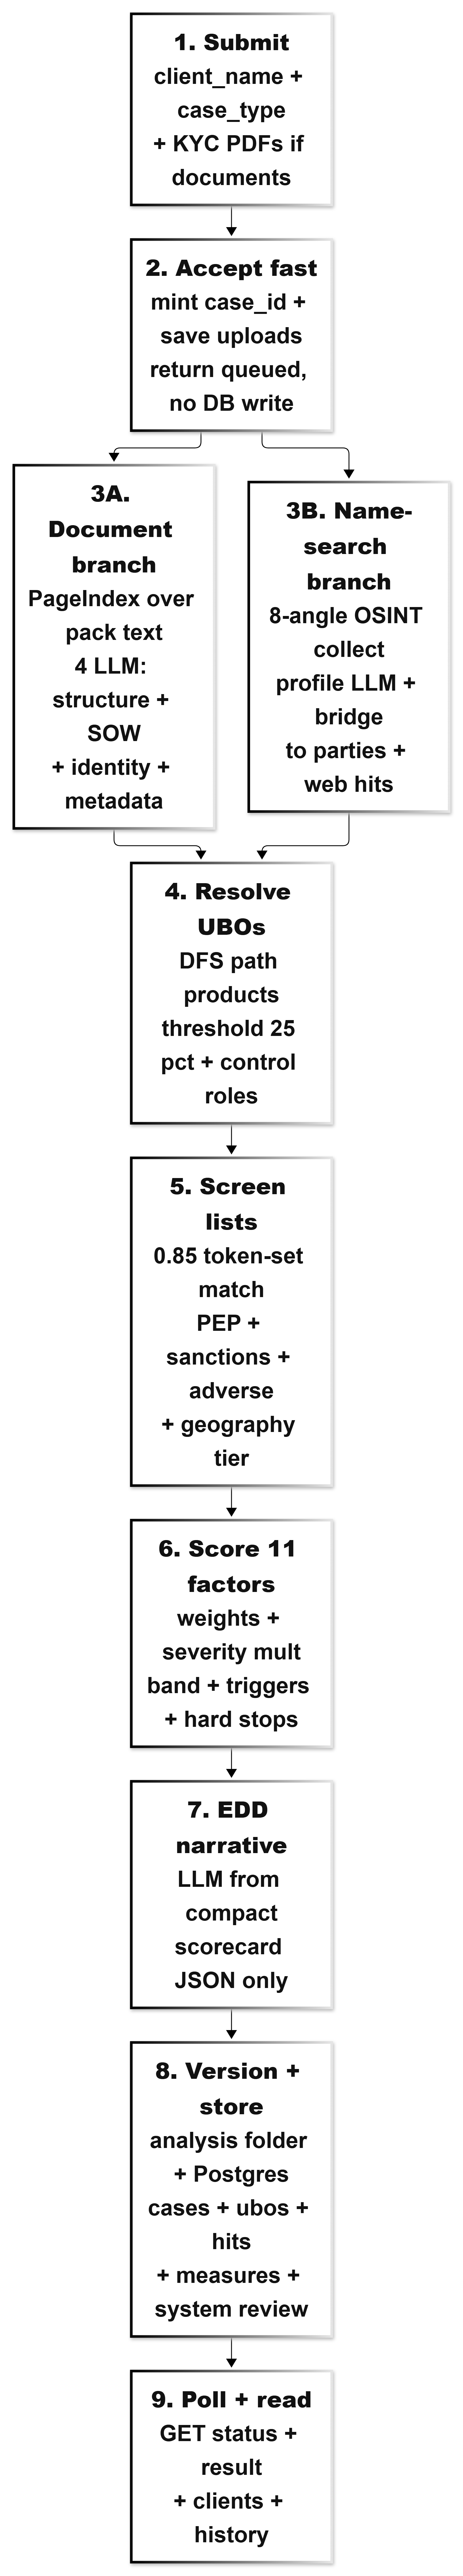
\includegraphics[width=\textwidth,height=0.85\textheight,keepaspectratio]{../diagrams/fraud_detection/01_flowchart_end-to-end-pipeline-diagram.png}
\caption{End-to-End Pipeline Diagram}
\label{fig:ch05_hni_onboarding-01-flowchart-end-to-end-pipeline-diagram}
\end{figure}

\speaker{Interviewer}{Why do both workflows converge after profile or document extraction?}

\speaker{Candidate}{Because ownership, screening, and risk-policy logic should not differ merely because the evidence arrived through a PDF or public search. The evidence structures may differ, but the final decision engine should be one deterministic implementation. That reduces policy drift.}

\subsection{Main Agents and Components}

\speaker{Candidate}{I would divide the system into these components:}

\subsubsection{Document Components}

\begin{itemize}[leftmargin=\speakwid]
\item Page loader and in-memory index.
\item Structure extraction agent.
\item Source-of-wealth extraction agent.
\item Identity verification extraction agent.
\item Case metadata extraction agent.
\end{itemize}
\subsubsection{OSINT Components}

\begin{itemize}[leftmargin=\speakwid]
\item Eight-angle query builder.
\item Web, news, and Wikipedia collectors.
\item Evidence deduplication.
\item Profile synthesis agent.
\item Profile-to-parties deterministic bridge.
\end{itemize}
\subsubsection{Deterministic Components}

\begin{itemize}[leftmargin=\speakwid]
\item Ownership and UBO resolver.
\item Watchlist and geography screening.
\item Risk scorecard.
\item Hard-stop and decision mapping.
\item Version calculation.
\end{itemize}
\subsubsection{Narrative Component}

\begin{itemize}[leftmargin=\speakwid]
\item EDD rationale generator using compact, authoritative scorecard JSON.
\end{itemize}
\subsubsection{Persistence and Interface Components}

\begin{itemize}[leftmargin=\speakwid]
\item FastAPI API.
\item Background wrappers.
\item S3 or ADLS upload storage.
\item Timestamped analysis storage in object storage.
\item Postgres tables for cases and derived outputs.
\item Web UI tabs for upload, name search, and historical KYC.
\end{itemize}

\speaker{Interviewer}{The pipeline is clear. Can you now justify the key decisions --- background execution, ownership resolution, and deterministic scoring?}

\medskip\hrule\medskip
\section{Deep Discussion on Pipeline Decisions}
\label{sec:ch05_hni_onboarding-5-deep-discussion-on-pipeline-decisions}

\subsection{Fast Accept and Background Execution}

\speaker{Interviewer}{Why does the API return before the assessment finishes?}

\speaker{Candidate}{The workflow can involve PDF page loading, multiple LLM calls, web searches, and EDD generation. Keeping the HTTP connection open would make timeouts likely. The API should generate a case ID, save uploads if needed, schedule the background wrapper, and return a queued response quickly.}

\speaker{Interviewer}{Does your design create a database row immediately?}

\speaker{Candidate}{No. Here is an important design detail. \texttt{POST /cases} creates a case ID and saves document uploads synchronously, but it does not write a processing row to Postgres before the background task. Until the task stores a result, the status endpoint synthesizes a processing response for the rowless case.}

\speaker{Interviewer}{Is that ideal?}

\speaker{Candidate}{It is simple but fragile. If the process crashes or the final database commit fails, the case can remain rowless and look like it is still processing. A stronger design would insert a \texttt{cases} row with \texttt{queued} status before scheduling the task.}

\speaker{Interviewer}{Is BackgroundTasks durable?}

\speaker{Candidate}{No. It runs inside the FastAPI process. A process restart can lose the task. For higher reliability, I would use a durable queue, idempotent job records, retry policies, and recovery for abandoned cases.}

\subsection{Document Page Index}

\speaker{Interviewer}{How does document evidence become searchable?}

\speaker{Candidate}{The document flow loads each PDF page with PyMuPDF text extraction. Empty pages are skipped, and pages are globally numbered across the document pack. An in-memory \texttt{PageIndex} creates embeddings, normalizes them, and supports cosine-similarity search.}

\speaker{Interviewer}{Why globally number pages?}

\speaker{Candidate}{Analysts need a stable reference across multiple PDFs. If the first PDF has pages 1--20 and the second starts at 21, an extracted party or source-of-wealth statement can cite one page namespace consistently.}

\speaker{Interviewer}{Is the page index persisted in Postgres?}

\speaker{Candidate}{No. My design declares \texttt{page\_chunks} but leaves that table unpopulated in the base flow. The page index is rebuilt for each request and exists in memory only.}

\speaker{Interviewer}{Are tool-calling agents using \texttt{search\_pages} and \texttt{get\_page}?}

\speaker{Candidate}{The tools are scaffolded but not bound to an LLM in the active flow. The extractors directly call \texttt{index.search()} and build evidence blocks. I would make that scope explicit in my proposal because the presence of a tools file does not mean an active agentic retrieval loop exists.}

\subsection{Document Structure Extraction}

\speaker{Interviewer}{What does the first document LLM do?}

\speaker{Candidate}{\texttt{extract\_structure} searches for ownership and relationship evidence and returns parties, ownership edges, relationships, and notes.}

\speakcont{Each party includes a stable ID such as \texttt{P1}, a name, party type, country or nationality when available, identifiers, declared PEP status, source page, and snippet. Edges represent ownership or control relationships. Relationships represent roles such as applicant, settlor, trustee, protector, beneficiary, director, shareholder, signatory, spouse, nominee, or UBO.}

\speaker{Interviewer}{How does the model avoid inventing a party?}

\speaker{Candidate}{The prompt instructs it to use only page evidence, never invent entities, preserve source snippets, and attach page numbers. Python then validates references, drops unknown endpoints, and tolerates malformed rows rather than trusting every model field blindly.}

\speaker{Interviewer}{Schema checks catch malformed rows, but how do you catch a well-formed yet wrong extraction --- for example, misclassified party types or dangling ownership edges?}

\speaker{Candidate}{That is exactly why the KYC workflow adds a correctness gate beyond schema, in \texttt{llm\_validation.py}. After \texttt{extract\_structure} returns, Python scores two things: party-type classification reports an estimated percent correct --- is each type in vocabulary, is the name grounded in the evidence block, is the ID shaped \texttt{P} plus a number --- and ownership extraction checks referential integrity plus percentages in the 0--100 range. This matters because a misclassified trust or a dangling edge would otherwise flow into UBO math and produce a plausible-looking but wrong beneficial owner. If confidence is below 0.50, Python lists the failed validations, appends them to the prompt through \texttt{build\_retry\_addendum}, and reinvokes the LLM once in a bounded retry. On failure it keeps the best attempt fail-soft so screening and scoring still run rather than blocking the case.}

\speakcont{For EDD purposes, the retry addendum might say which party types were invalid or which edges pointed at unknown IDs, so the model corrects grounding instead of repeating the same mistake.}

\subsection{Source of Wealth}

\speaker{Interviewer}{Why is source of wealth separate from structure extraction?}

\speaker{Candidate}{It has a different search pattern and different output. Structure extraction asks who owns or controls whom. Source-of-wealth extraction asks how a principal obtained wealth and whether the declaration is corroborated. Separating them gives each task a focused prompt and makes missing evidence explicit.}

\speaker{Interviewer}{What if the source of wealth is simply ``private investments'' without supporting documents?}

\speaker{Candidate}{Python should preserve the declared signal but mark corroboration as missing or false. The scoring engine can then activate the opaque-source-of-wealth factor according to policy.}

\subsection{Identity Verification}

\speaker{Interviewer}{What identity information should be extracted?}

\speaker{Candidate}{For each relevant party, the agent can record document type, document number, verified or certified status, gaps such as expired documents or missing proof of address, and source page.}

\speaker{Interviewer}{Why should identity gaps affect risk?}

\speaker{Candidate}{A missing or unverifiable identity document is not necessarily fraud, but it creates a compliance gap. It should contribute to the risk score or EDD information requirements without being treated as a sanctions match.}

\subsection{Name-Based OSINT Collection}

\speaker{Interviewer}{Explain the name-search workflow in depth.}

\speaker{Candidate}{The system creates a \texttt{SubjectSeed} from the client name and optional context. The collector searches eight dimensions:}

\begin{enumerate}[leftmargin=\speakwid]
\item Biography.
\item Professional history.
\item Company performance.
\item Adverse media.
\item PEP indicators.
\item Social and behavioral information.
\item Relationships.
\item Wealth and source of wealth.
\end{enumerate}
\speakcont{It uses web search, news search, and Wikipedia where available. Results are stored as snippets with dimension, query, title, URL, source, and publication date when available. Duplicate results are removed by URL or normalized snippet.}

\speaker{Interviewer}{Why eight angles instead of one broad query?}

\speaker{Candidate}{A single broad query tends to overrepresent popular or recent pages and can miss important categories such as relationships, adverse media, or source of wealth. Separate dimensions make collection more systematic and allow the profile model to reason about gaps.}

\speaker{Interviewer}{What if the name is common?}

\speaker{Candidate}{Name ambiguity is one of the highest risks. The seed should include location, nationality, age, employer, aliases, or known companies when available. The profile must report disambiguation confidence. Low confidence should be clearly surfaced to the analyst and should make web-derived findings less trusted.}

\subsection{Web Evidence Credibility}

\speaker{Interviewer}{Should one online article be enough to mark a client as high risk?}

\speaker{Candidate}{No. Web evidence is supporting evidence, not equivalent to a curated sanctions match. My design discounts web adverse findings by one severity level, caps a single web source at medium, and allows multiple consistent high-severity web findings to restore high severity. This prevents one unverified article from dominating the score.}

\speaker{Interviewer}{What if the article is from a highly credible regulator?}

\speaker{Candidate}{My design does not fully model source credibility beyond the web-source treatment. I would add source-quality metadata and allow trusted official sources to receive stronger weight while still preserving human review.}

\speaker{Interviewer}{Does the same correctness idea apply to the name-search profile, where the model could invent adverse findings or cite nothing?}

\speaker{Candidate}{Yes, and it matters even more there because a false adverse claim can trigger EDD or escalation. After \texttt{synthesize\_profile} returns \texttt{Profile360}, Python runs \texttt{score\_profile\_suggestion}: disambiguation must be \texttt{low}, \texttt{medium}, or \texttt{high}; adverse severity must use the controlled vocabulary; summaries must be non-empty; and every adverse URL must already exist in the collected evidence, otherwise it is flagged as \texttt{uncited\_adverse}. An empty ownership graph scores 0.55 because no edges can be legitimate for a person with no corporate footprint. Below 0.50 confidence the failed checks are appended to the prompt and the profile is reinvoked once. For the analyst this means a single uncited fraud allegation cannot quietly become a high-severity hit --- it is either grounded or surfaced as a gap.}

\speakcont{The gate sits on top of strict input limits that also control quality: at most 120 numbered evidence lines per profile call with snippets truncated to about 280 characters, so the model reasons over deduplicated web, news, and Wikipedia snippets rather than unbounded text.}

\subsection{UBO Resolution}

\speaker{Interviewer}{Now explain beneficial ownership. This is usually where mistakes happen.}

\speaker{Candidate}{The resolver first identifies the applicant. It then traverses ownership edges using depth-first search. For each ownership path, it multiplies percentages across the chain. If an individual owns 60 percent of Holding A and Holding A owns 50 percent of Applicant B, the effective ownership is 30 percent.}

\speakcont{The resolver qualifies a UBO when effective ownership is at least the configured threshold, normally 25 percent, or when the party has a control role such as settlor, trustee, protector, director, or signatory. If no person qualifies, the system falls back to a senior managing official when available.}

\speaker{Interviewer}{What happens when a percentage is missing?}

\speaker{Candidate}{The path is retained as control evidence, but a missing percentage is treated as zero for effective ownership calculation in my design. My design must not invent a percentage. I would represent unknown ownership separately instead of treating it numerically as zero.}

\speaker{Interviewer}{What if the structure contains a cycle?}

\speaker{Candidate}{The DFS detects the cycle, skips the recursive path, records that circular ownership was observed, and exposes it as an opacity and scoring signal.}

\speaker{Interviewer}{How do you detect layering?}

\speaker{Candidate}{The resolver records path depth. A depth of three or more ownership links activates layering and can also activate the complex-structure factor. Larger depths can receive higher severity.}

\subsection{Deterministic Screening}

\speaker{Interviewer}{How does watchlist matching work?}

\speaker{Candidate}{Names are normalized to lowercase alphanumeric tokens. Common corporate and honorific stopwords are removed. The system calculates token-set similarity. A perfect token-set match scores 1.0; otherwise it calculates intersection divided by union. Matches at or above 0.85 are retained.}

\speakcont{The system checks sanctions, PEP, adverse-media reference data, declared PEP status, and jurisdiction risk. The result is a structured \texttt{WatchlistHit} or \texttt{GeographyHit} with party, matched name, score, tier, details, and source.}

\speaker{Interviewer}{Why use token similarity instead of an LLM?}

\speaker{Candidate}{Screening must be reproducible and resistant to prompt variability. Deterministic matching is easier to test and explain. More advanced production matching could add transliteration, aliases, date of birth, nationality, and specialist entity-resolution models, but the final match decision should remain controlled and reviewable.}

\subsection{Deterministic Risk Scorecard}

\speaker{Interviewer}{Walk me through the scorecard.}

\speaker{Candidate}{The scorecard has eleven factors:}

\begin{itemize}[leftmargin=\speakwid]
\item Sanctions.
\item PEP.
\item Adverse media.
\item Opaque source of wealth.
\item Nominee involvement.
\item Bearer shares.
\item High-risk geography.
\item Complex structure.
\item Layering.
\item Identity-verification gap.
\item Offshore exposure.
\end{itemize}
\speakcont{Each factor has a weight. A severity multiplier is applied: low equals 0.5, medium equals 1.0, and high equals 1.5. Contributions are summed and capped at 100.}

\speakcont{The bands are:}

\begin{itemize}[leftmargin=\speakwid]
\item Score at least 50: HIGH.
\item Score at least 25 and below 50: MEDIUM.
\item Below 25: LOW.
\end{itemize}
\speakcont{Sanctions and prohibited jurisdictions create hard stops and produce a PROHIBITED band. The decision mapping is:}

\begin{itemize}[leftmargin=\speakwid]
\item Hard stop or PROHIBITED: DECLINE.
\item HIGH: ESCALATE\_MLRO.
\item MEDIUM or EDD required: APPROVE\_WITH\_EDD.
\item Otherwise: APPROVE\_STANDARD\_CDD.
\end{itemize}
\speaker{Interviewer}{Why not let the LLM decide the risk band from the evidence?}

\speaker{Candidate}{Because a risk band is a policy decision. It should be reproducible, testable, and consistent across cases. The LLM can summarize evidence, but Python should apply weights, thresholds, hard stops, and decision mapping.}

\speaker{Interviewer}{You said each factor has a weight. What are the actual weights, and why should I care as a compliance owner?}

\speaker{Candidate}{The weights encode policy judgment, and my proposal states them exactly: sanctions 100.0, PEP 30.0, adverse media 28.0, opaque source of wealth 26.0, nominee 24.0, bearer shares 24.0, high-risk geography 20.0, complex structure 16.0, layering 16.0, identity-verification gap 14.0, and offshore 10.0, with severity multipliers low 0.5, medium 1.0, and high 1.5, summed and capped at 100. A sanctions weight of 100.0 is effectively a hard stop on its own, while offshore at 10.0 can only nudge a case. EDD is required when any trigger from PEP, adverse media, high-risk geography, opaque source of wealth, complex structure, nominee, or bearer shares is present, or when the band is MEDIUM or HIGH.}

\speakcont{Operationally the run also emits a \texttt{metrics} record --- document counts, \texttt{llm\_calls} of 5 plus one optional Q\&A turn for document cases and 2 plus one for name cases, party and UBO counts or evidence-item counts, band, decision, and latency in milliseconds --- plus four markdown reasoning strings for document cases, so audit and capacity planning see the same numbers the scorecard used.}

\subsection{EDD Narrative Generation}

\speaker{Interviewer}{Where does the LLM come back into the flow?}

\speaker{Candidate}{After the deterministic scorecard is complete. The EDD agent receives compact scorecard JSON containing the applicant, score, band, decision, triggers, UBOs, structure statistics, watchlist hits, and geography hits. It does not receive raw documents or unconstrained web content in this final step.}

\speakcont{It writes a risk summary, key drivers, EDD measures, information still required, and watch items. The prompt explicitly says the scorecard is authoritative and that the model must not recompute or override the decision.}

\speaker{Interviewer}{Why pass only compact scorecard JSON?}

\speaker{Candidate}{It narrows the LLM's role to explanation. The final narrative cannot silently calculate a different risk score or invent a new hard stop from raw text. That improves consistency and auditability.}

\speaker{Candidate}{Before we leave scoring, may we unpack the deterministic core --- effective ownership math, jurisdiction tiers, and hard-stop logic?}

\medskip\hrule\medskip
\section{Deterministic Fraud and KYC Risk Core}
\label{sec:ch05_hni_onboarding-6-deterministic-fraud-and-kyc-risk-core}

\speaker{Interviewer}{Now go deeper into the deterministic engine. I want to understand the calculations.}

\subsection{Applicant Resolution}

\speaker{Candidate}{The system resolves the applicant in this order:}

\begin{enumerate}[leftmargin=\speakwid]
\item Use the explicit applicant party ID from case metadata.
\item Use a party with the \texttt{applicant} relationship.
\item Infer a single ownership sink when possible.
\item Prefer an appropriate non-individual entity when the structure is ambiguous.
\item Fall back to the first party only as a final design fallback.
\end{enumerate}
\speakcont{This is important because a trust or holding company may be the applicant even when an individual is the ultimate owner.}

\subsection{Effective Ownership}

For every ownership path, the resolver multiplies percentages along the path:

i.effective ownership =

\[
\prod_{i=1}^{n} \frac{p_i}{100} \times 100
\]

For example, if Person A owns 80 percent of Company B and Company B owns 40 percent of Applicant C:

\[
80\% \times 40\% = 32\%
\]

Person A qualifies as an ownership-based UBO when the result meets the threshold.

\subsection{Control-Based UBOs}

\speaker{Candidate}{Ownership is not the only way someone can control a structure. Settlor, trustee, protector, director, and signatory roles can qualify a party for control-based UBO treatment even when the percentage is unknown.}

\speakcont{The system stores the basis as \texttt{control} and records the control roles. That gives the analyst a clear explanation of why the party was identified.}

\subsection{Fallback Senior Managing Official}

\speaker{Interviewer}{What if no person reaches the 25 percent threshold and no explicit control role is available?}

\speaker{Candidate}{The resolver selects a suitable individual director as a senior managing official fallback. This should not be confused with proving beneficial ownership. It is a compliance fallback that ensures the case still has an accountable natural person for review.}

\subsection{Opacity and Structure Signals}

The ownership engine also calculates:

\begin{itemize}[leftmargin=\speakwid]
\item Number of entities.
\item Number of parties.
\item Maximum layering depth.
\item Presence of nominee parties or roles.
\item Bearer-share mentions.
\item Circular ownership.
\end{itemize}
These are not final decisions by themselves, but they become evidence for complex-structure, layering, nominee, and bearer-share factors.

\subsection{Watchlist and Jurisdiction Matching}

\speaker{Candidate}{Screening produces watchlist hits and geography hits. Sanctions hits are treated as hard stops. PEP hits contribute according to tier. Adverse-media hits contribute based on source and severity. High-risk jurisdictions activate geography and potentially offshore factors. Prohibited jurisdictions produce a hard stop.}

\subsection{Score Calculation}

The score is computed as:

\[
\text{raw score} = \sum_i \text{weight}_i \times \text{severity multiplier}_i
\]

Then:

\[
\text{normalized score} = \min(100, \text{raw score})
\]

The scorecard stores every active factor, its weight, severity, contribution, evidence, and pages. This is more useful than storing only the final number.

\subsection{Scorecard Decision Diagram}

\begin{figure}[htbp]
\centering

\includegraphics[width=\textwidth,height=0.85\textheight,keepaspectratio]{../diagrams/fraud_detection/02_flowchart_scorecard-decision-diagram.png}
\caption{Scorecard Decision Diagram}
\label{fig:ch05_hni_onboarding-02-flowchart-scorecard-decision-diagram}
\end{figure}

\speaker{Interviewer}{The scorecard logic is clear. How does the EDD narrative explain the score, triggers, and missing information?}

\medskip\hrule\medskip
\section{EDD Narrative and Q\&A}
\label{sec:ch05_hni_onboarding-7-edd-narrative-and-q-a}

\speaker{Interviewer}{Explain the narrative and question-answering behavior.}

\speaker{Candidate}{The EDD rationale is generated after scoring. The model receives a compact authoritative representation, not raw documents. It returns:}

\begin{itemize}[leftmargin=\speakwid]
\item Risk summary.
\item Key drivers.
\item EDD measures.
\item Information required.
\item Watch items.
\end{itemize}
\speakcont{For example, if the system finds an opaque source of wealth and a high-risk jurisdiction, the narrative might recommend independent source-of-wealth corroboration, senior compliance approval, and enhanced transaction monitoring.}

\speaker{Interviewer}{Can the narrative change the decision from \texttt{ESCALATE\_MLRO} to \texttt{APPROVE\_STANDARD\_CDD}?}

\speaker{Candidate}{No. The narrative is explanatory. The deterministic scorecard and hard-stop logic remain authoritative.}

\speaker{Interviewer}{How does Q\&A work?}

\speaker{Candidate}{The in-process Q\&A functions receive compact case JSON and a user question. The document flow answers from applicant, decision, band, score, triggers, UBOs, active factors, and watchlist hits. The name flow also includes profile information, relationships, companies, adverse findings, PEP indicators, wealth, behavioral summary, and data gaps.}

\speakcont{The system should admit when the supplied information does not answer the question. It should not invent facts or present public-web information as confirmed identity.}

\speaker{Interviewer}{Is Q\&A available through the production HTTP API?}

\speaker{Candidate}{No. My design exposes no question endpoint on the HTTP API. Q\&A exists in the agent and development workflows. I would note that as an open gap.}

\speaker{Candidate}{With EDD and Q\&A covered, shall we step back to the high-level architecture and the trust boundary between the LLM and the deterministic risk engine?}

\medskip\hrule\medskip
\section{High-Level Design}
\label{sec:ch05_hni_onboarding-8-high-level-design}

\speaker{Interviewer}{Please give me the high-level architecture.}

\speaker{Candidate}{My design is a single FastAPI application with two workflow wrappers and shared risk services.}

\subsection{Architecture Components}

\begin{enumerate}[leftmargin=\speakwid]
\item Web UI with Document Upload, Name Search, and Historical KYC tabs.
\item FastAPI service exposing case creation, status, result, client list, and history endpoints.
\item In-process \texttt{BackgroundTasks} for asynchronous execution.
\item S3 or ADLS object storage under the generated case-ID prefix.
\item Timestamped analysis folders for completed results.
\item In-memory NumPy page index for document evidence retrieval.
\item OpenAI-compatible LLM gateway for extraction, profile synthesis, EDD, and Q\&A.
\item OSINT adapters for DuckDuckGo, Google, Wikipedia, and news search.
\item Deterministic ownership, screening, and scoring modules.
\item Postgres tables for cases and derived UBO, watchlist, EDD, and review records.
\end{enumerate}
\subsection{High-Level Architecture Diagram}

\begin{figure}[htbp]
\centering
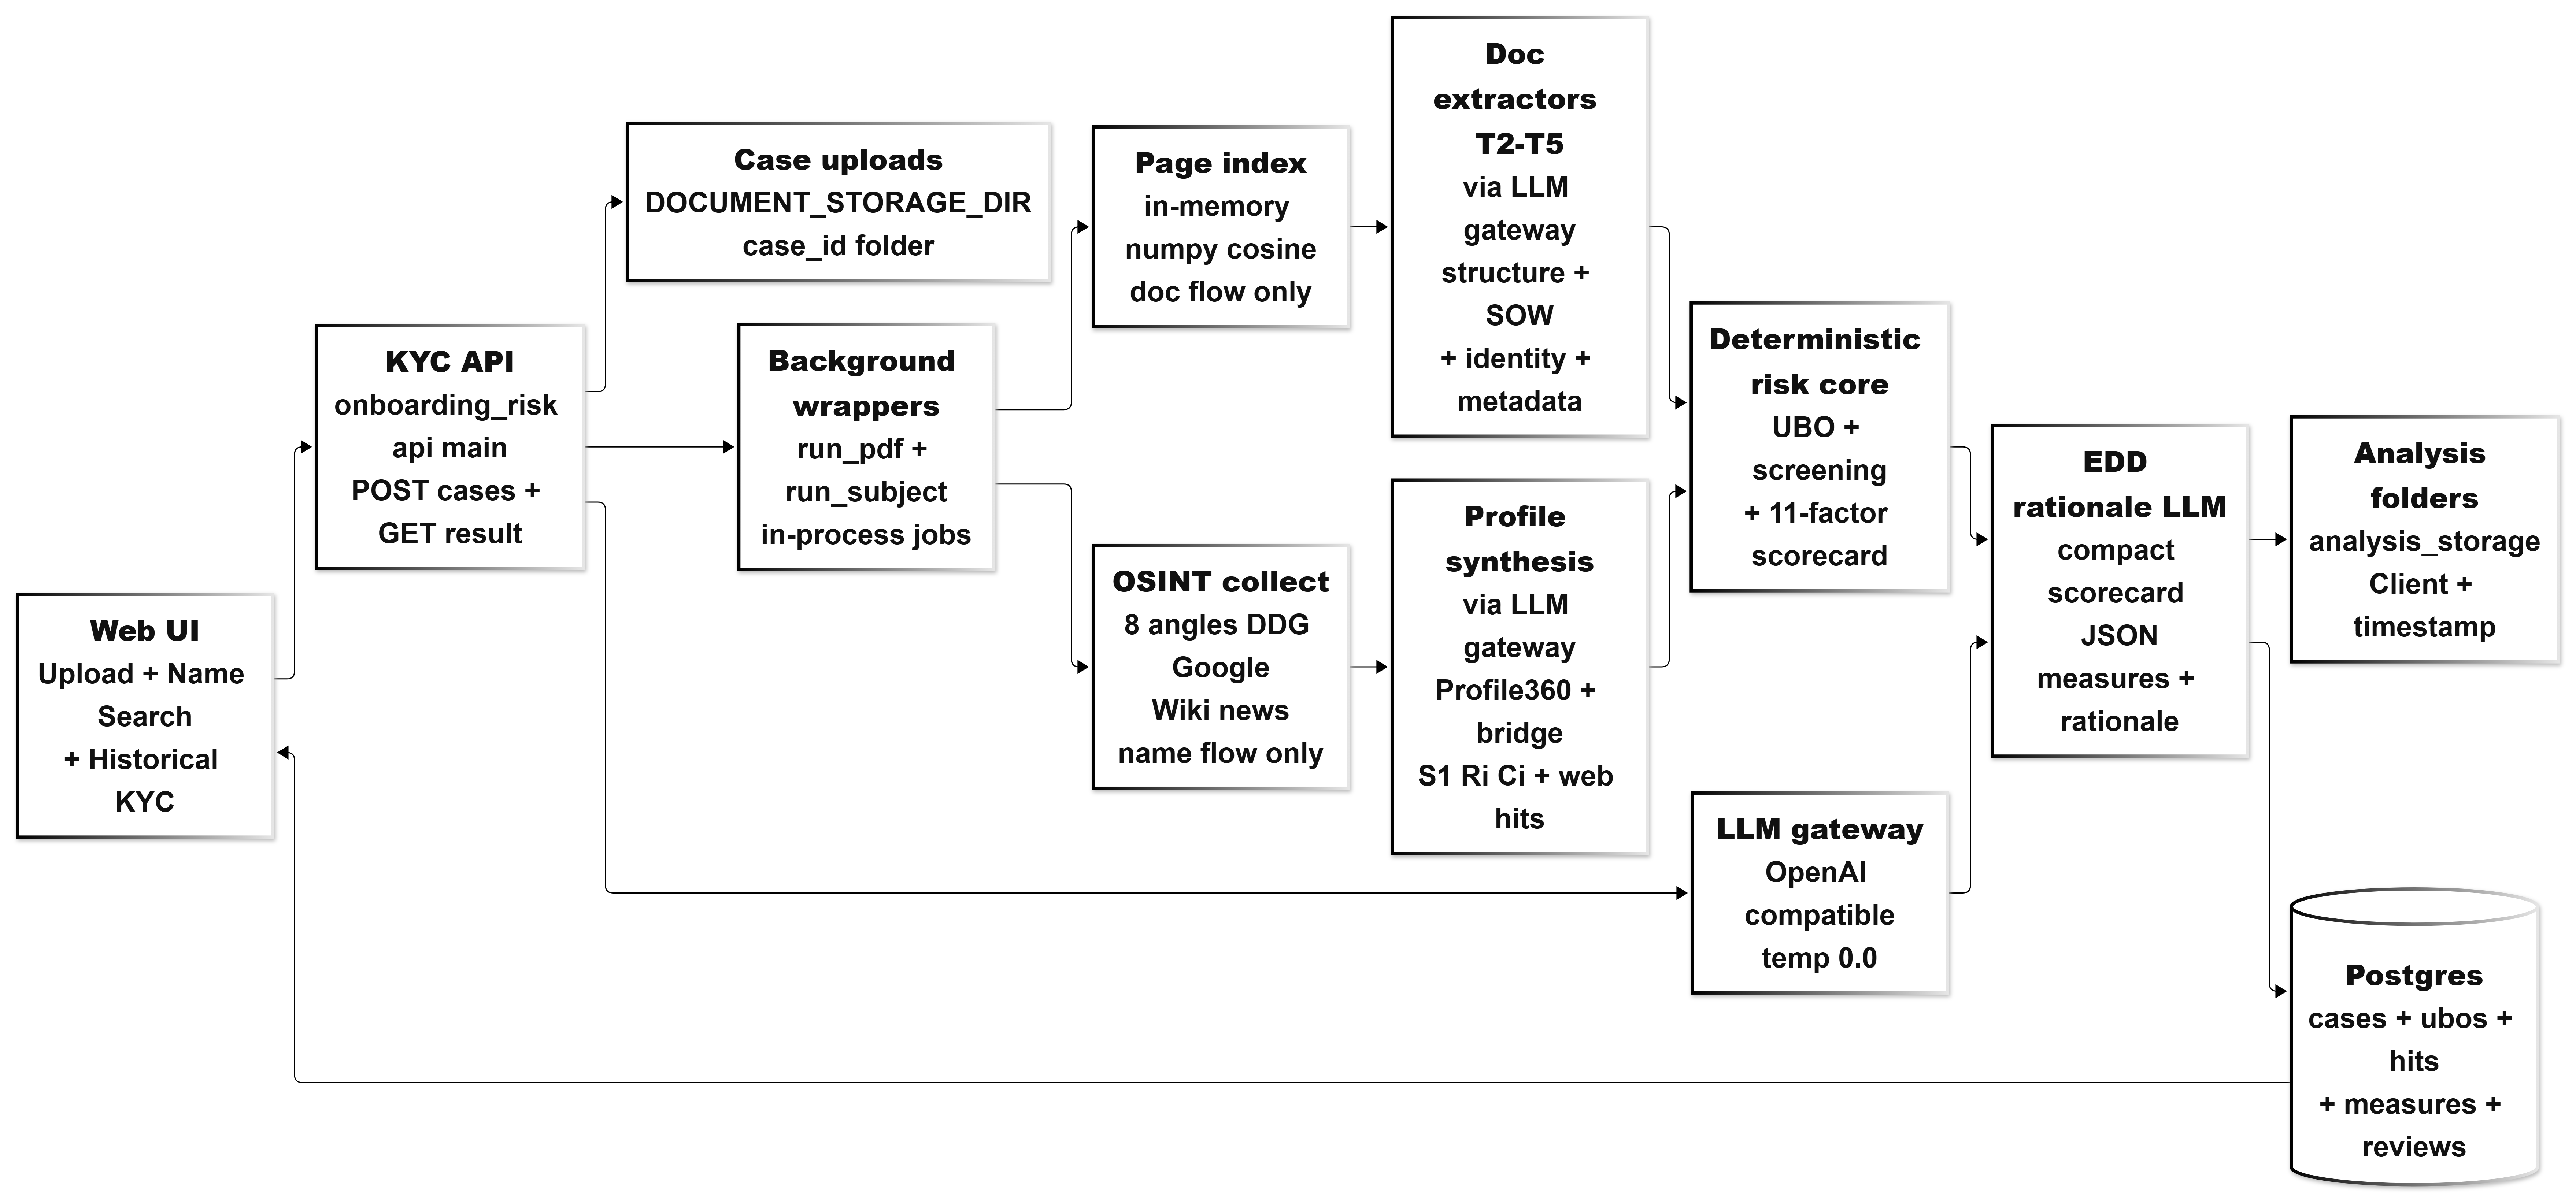
\includegraphics[width=\textwidth,height=0.85\textheight,keepaspectratio]{../diagrams/fraud_detection/03_flowchart_high-level-architecture-diagram.png}
\caption{High-Level Architecture Diagram}
\label{fig:ch05_hni_onboarding-03-flowchart-high-level-architecture-diagram}
\end{figure}

\speaker{Interviewer}{Why not split document extraction, OSINT, scoring, and EDD into separate microservices immediately?}

\speaker{Candidate}{My design keeps a tightly coupled workflow and the first goal is clarity. A modular single service is easier to test and deploy. We can split components later when independent scaling, security boundaries, or team ownership justify it. Splitting too early would increase operational complexity without solving the main bottleneck.}

\speaker{Interviewer}{Where is the trust boundary between the LLM and the risk engine?}

\speaker{Candidate}{The LLM produces evidence candidates and narrative text. The deterministic engine validates and reinterprets those outputs. The LLM cannot directly set the band, score, hard-stop reason, UBO percentage, or final decision.}

\speaker{Interviewer}{High-level shape makes sense. Walk me through the low-level KYC request lifecycle from submission to versioned result?}

\medskip\hrule\medskip
\section{Low-Level Design}
\label{sec:ch05_hni_onboarding-9-low-level-design}

\speaker{Interviewer}{Now go into the low-level design. I want to understand the request lifecycle and modules.}

\subsection{Request Lifecycle}

\begin{itemize}[leftmargin=\speakwid]
\item \texttt{POST /cases} accepts multipart form data.
\item A UUID case ID is generated.
\item Document uploads are saved under the case directory.
\item A \texttt{SubjectSeed} is built for name search.
\item A background wrapper is scheduled.
\item The API returns \texttt{queued} quickly.
\item The wrapper runs the selected workflow.
\item The deterministic tail calculates UBOs, screening, score, and decision.
\item EDD rationale is generated.
\item Versioned analysis files are saved.
\item Postgres records are inserted in one final transaction.
\end{itemize}

\speaker{Interviewer}{Can you pin down the API surface and the exact retrieval contracts the modules rely on?}

\speaker{Candidate}{There are eight endpoints: \texttt{GET /} serves the web UI, \texttt{GET /health} returns healthy plus timestamp for probes, \texttt{POST /cases} accepts multipart client name, case type, optional description, and files and returns queued without writing a row, \texttt{GET /cases/\{id\}} fetches the case and returns 404 while rowless, \texttt{GET /cases/\{id\}/status} synthesizes processing at 0.5 progress until a row exists and then reports completed or failed at 1.0 or 0.0, \texttt{GET /cases/\{id\}/result} prefers relational UBO, hit, and measure rows with a \texttt{raw\_result} fallback and returns 404 when missing or 400 when not completed, plus \texttt{GET /clients} and \texttt{GET /clients/\{name\}/history} for historical KYC. The description field is accepted but not persisted to \texttt{cases.description} in my design, so analysts should not rely on it for audit.}

\speakcont{Retrieval is equally pinned: structure uses top-8 pages for a beneficial-owner and trust-deed query, source of wealth and identity each use top-6 pages for their respective queries, and metadata uses top-4 pages for an application-form query, pasted as page blocks with party directories where needed. Structure snippets truncate at 300 characters and source-of-wealth narratives at 600, edges with unknown or self endpoints are dropped, and percentages are coerced to float or null. Supporting modules are \texttt{llm\_validation.py} for the gates above, \texttt{db/persist\_graph.py} for graph persistence, and four offline tests in \texttt{tests/test\_llm\_validation.py} covering gate scoring and retry without network access.}
\subsection{Document Workflow Modules}

\begin{itemize}[leftmargin=\speakwid]
\item \texttt{agent\_graph.py} orchestrates document cases.
\item \texttt{extraction.py} contains the four document extraction calls.
\item \texttt{doc\_index.py} loads PDF pages and performs cosine search.
\item \texttt{ownership.py} resolves UBOs.
\item \texttt{screening.py} matches watchlists and jurisdictions.
\item \texttt{scoring.py} applies the eleven-factor scorecard.
\item \texttt{edd.py} generates the EDD rationale.
\item \texttt{storage.py} saves timestamped analysis files.
\item \texttt{db/models.py} defines SQLAlchemy tables.
\end{itemize}
\subsection{Name-Search Workflow Modules}

\begin{itemize}[leftmargin=\speakwid]
\item \texttt{subject\_graph.py} orchestrates name cases.
\item \texttt{osint/collect.py} builds and executes eight-angle searches.
\item \texttt{osint/search.py} wraps web, news, Google, DuckDuckGo, and Wikipedia access.
\item \texttt{osint/profile.py} synthesizes \texttt{Profile360}.
\item \texttt{profile\_to\_parties} maps the profile into deterministic party structures.
\item Shared ownership, screening, scoring, EDD, and persistence logic completes the case.
\end{itemize}
\subsection{Background Wrapper Behavior}

\speaker{Interviewer}{What does the wrapper do if a case fails halfway through?}

\speaker{Candidate}{The wrapper catches the exception and writes a minimal failed case row. The status endpoint then reports \texttt{failed}, and the result endpoint rejects incomplete cases. This protects the API from returning an unhandled server error, although I would improve error diagnostics and recovery in my design.}

\speaker{Interviewer}{What if OSINT is unavailable?}

\speaker{Candidate}{Name search should still complete with an empty or near-empty profile, subject to the available deterministic evidence. OSINT failure should not be treated as proof of low risk. The result should expose missing public evidence and lower confidence.}

\speaker{Interviewer}{What if the document page has no text?}

\speaker{Candidate}{The page is skipped during indexing. If the complete pack has no usable text, the document workflow fails rather than continuing with false confidence.}

\subsection{Versioning}

\speaker{Interviewer}{Explain client-history versioning.}

\speaker{Candidate}{When a completed assessment is saved, the system finds previous cases for the same client, marks the previous latest case as not latest, and assigns the new case the next analysis version. The Historical KYC endpoint returns versions newest first.}

\speaker{Interviewer}{What if two assessments for the same client finish at the same time?}

\speaker{Candidate}{My design provides no strong concurrency guarantee around version assignment. I would use a transaction lock, unique constraint, or database sequence scoped by client.}

\subsection{Storage Behavior}

\speaker{Interviewer}{Where are files stored?}

\speaker{Candidate}{Uploads are stored in S3 or ADLS under \texttt{<case\_id>/} prefixes. Completed results are written under versioned \texttt{<SafeClient>\_<timestamp>/} prefixes, with metadata and a full analysis result JSON. The storage manager sanitizes client names for key safety.}

\speaker{Interviewer}{How do documents and artifacts map to storage in your design?}

\speaker{Candidate}{Yes. S3 or ADLS is authoritative for documents and analysis artifacts, and the database stores durable object URIs. The deployment stays a single service for simplicity, not because files cannot be shared.}

\speaker{Interviewer}{Storage is clear. Can you detail the data model --- cases, UBOs, watchlist hits, and historical KYC versions?}

\medskip\hrule\medskip
\section{Data Modeling}
\label{sec:ch05_hni_onboarding-10-data-modeling}

\speaker{Interviewer}{Now I want the data model in detail. Include the entity relationship diagram and the table structures.}

\speaker{Candidate}{The core design is case-centric. A case represents one onboarding assessment version. Derived results such as UBOs, watchlist hits, EDD measures, and system review rows point back to that case.}

\speakcont{By design, some richer entities are declared in SQLAlchemy and left unpopulated in the base flow. Parties and ownership edges live inside \texttt{raw\_result} and analysis files, while derived UBO and screening results are stored relationally.}

\subsection{Entity Relationship Diagram}

\begin{figure}[htbp]
\centering
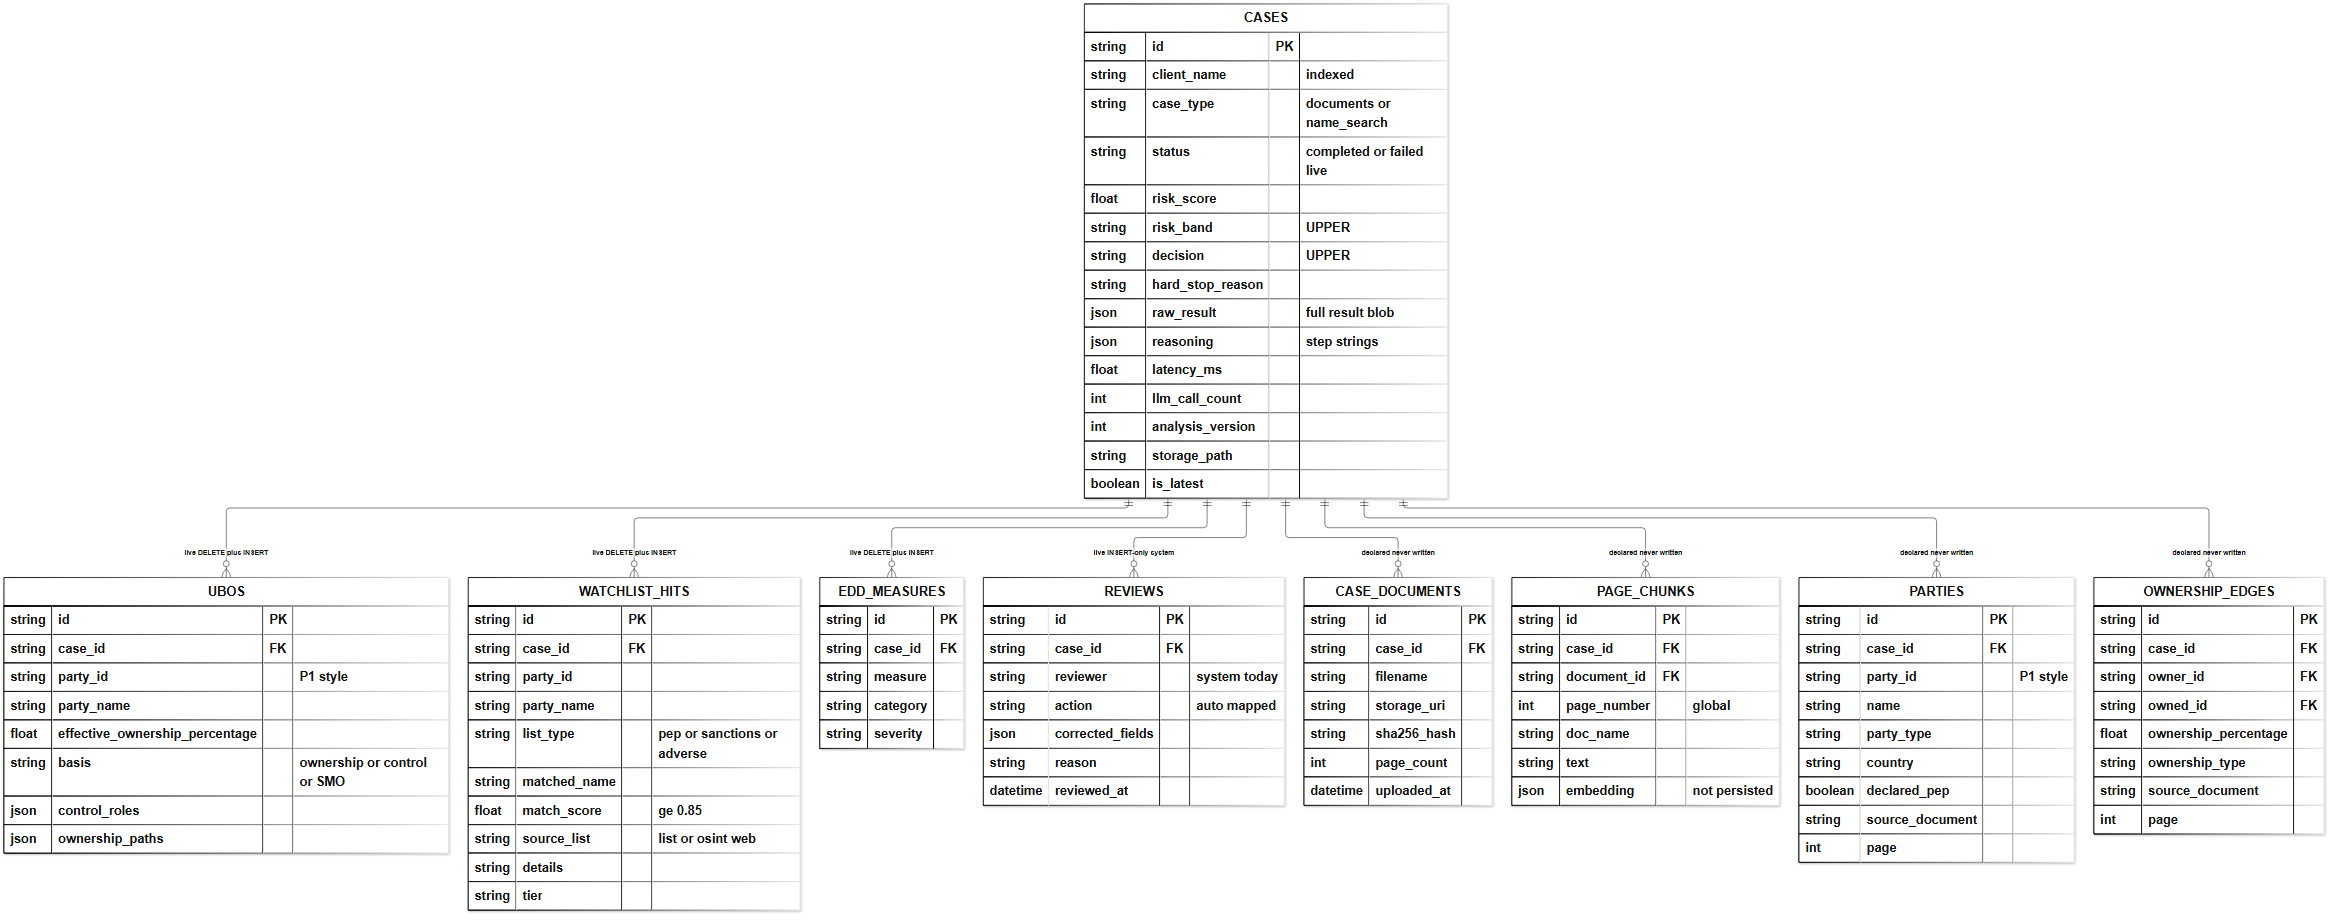
\includegraphics[width=\textwidth,height=0.85\textheight,keepaspectratio]{../diagrams/fraud_detection/04_erDiagram_10-1-entity-relationship-diagram.png}
\caption{Entity Relationship Diagram}
\label{fig:ch05_hni_onboarding-04-erdiagram-10-1-entity-relationship-diagram}
\end{figure}

\subsection{Live and Declared Tables}

\begin{xltabular}{\textwidth}{>{\raggedright\arraybackslash}X >{\raggedright\arraybackslash}X >{\raggedright\arraybackslash}X}
\caption{Live and Declared Tables}\label{tab:ch05_hni_onboarding-10-2-live-and-declared-tables-1}\\
\hline
\textbf{Table} & \textbf{Current status} & \textbf{Main purpose} \\
\hline
\endfirsthead
\caption[]{Live and Declared Tables (continued)}\\
\hline
\textbf{Table} & \textbf{Current status} & \textbf{Main purpose} \\
\hline
\endhead
\texttt{cases} & Live & Stores assessment status, risk summary, version, raw result, and storage path \\
\texttt{ubos} & Live & Stores resolved beneficial owners after each completed assessment \\
\texttt{watchlist\_hits} & Live & Stores sanctions, PEP, and adverse-media hits \\
\texttt{edd\_measures} & Live & Stores recommended EDD actions \\
\texttt{reviews} & Live, system-generated & Stores an automatic system review row; no human review endpoint exists \\
\texttt{case\_documents} & Declared but not populated & Intended document metadata table; current uploads are stored in S3 or ADLS \\
\texttt{page\_chunks} & Declared but not populated & Intended persistent page-index table; current index is in memory \\
\texttt{parties} & Declared but not populated & Intended relational party table; parties currently remain in JSON \\
\texttt{ownership\_edges} & Declared but not populated & Intended relational ownership table; edges currently remain in JSON \\
\hline
\end{xltabular}

\speaker{Candidate}{Can we go deeper on persistence? I want those graph tables populated relationally from the start, with UBO paths, documents, and ownership queryable per case.}

\speaker{Interviewer}{Please do. What is stored relationally?}

\speaker{Candidate}{All nine tables are written on every save. \texttt{persist\_case\_graph()} writes \texttt{case\_documents}, \texttt{page\_chunks}, \texttt{parties}, and \texttt{ownership\_edges} on every save with idempotent DELETE plus INSERT, and \texttt{classify\_edd\_measure()} fills \texttt{edd\_measures.category} and \texttt{severity} instead of leaving them reserved. For KYC work this matters because UBO paths, watchlist hits, and EDD actions are queryable per case, while the full extraction evidence remains in \texttt{raw\_result} and versioned analysis files for lineage. Best-effort page-chunk rows are capped at about 500 per case so a very large pack does not flood the table.}

\speakcont{Concretely, \texttt{category} is one of monitoring, documentation, approval, screening, or other, and \texttt{severity} is high when the measure mentions sanctions, PEP, prohibit, decline, escalate, or freeze, otherwise medium --- so an MLRO can filter high-severity monitoring actions without parsing free text.}

\subsection{Physical Table Structures}

\subsubsection{Table: \texttt{cases}}

\begin{xltabular}{\textwidth}{>{\raggedright\arraybackslash}X >{\raggedright\arraybackslash}X >{\raggedright\arraybackslash}X >{\raggedright\arraybackslash}X}
\caption{Table: cases}\label{tab:ch05_hni_onboarding-table-cases-2}\\
\hline
\textbf{Column} & \textbf{Type} & \textbf{Key / nullable} & \textbf{Description} \\
\hline
\endfirsthead
\caption[]{Table: cases (continued)}\\
\hline
\textbf{Column} & \textbf{Type} & \textbf{Key / nullable} & \textbf{Description} \\
\hline
\endhead
\texttt{id} & String & PK & Unique case identifier \\
\texttt{client\_name} & VARCHAR(255) & Indexed, not null & Client or applicant name \\
\texttt{case\_type} & VARCHAR(32) & Not null & \texttt{documents} or \texttt{name\_search} \\
\texttt{description} & TEXT & Nullable & Optional purpose note \\
\texttt{status} & VARCHAR(32) & Not null & Live values are mainly \texttt{completed} and \texttt{failed} \\
\texttt{model\_name} & VARCHAR(128) & Nullable & Model metadata; not currently populated consistently \\
\texttt{embed\_model\_name} & VARCHAR(128) & Nullable & Embedding model metadata \\
\texttt{risk\_score} & FLOAT & Nullable & Normalized score from 0 to 100 \\
\texttt{risk\_band} & VARCHAR(32) & Nullable & Stored uppercase in the database \\
\texttt{decision} & VARCHAR(64) & Nullable & Stored uppercase in the database \\
\texttt{hard\_stop\_reason} & TEXT & Nullable & Sanctions or prohibited-jurisdiction reason \\
\texttt{raw\_result} & JSON & Nullable & Full serialized assessment \\
\texttt{reasoning} & JSON & Nullable & Pipeline reasoning or step trace \\
\texttt{latency\_ms} & FLOAT & Nullable & End-to-end processing latency \\
\texttt{llm\_call\_count} & INTEGER & Nullable & Number of LLM calls \\
\texttt{requested\_by} & VARCHAR(128) & Nullable & Requester identity; currently defaults rather than using authentication \\
\texttt{requested\_at} & DATETIME & Not null & Case creation time \\
\texttt{completed\_at} & DATETIME & Nullable & Completion time \\
\texttt{analysis\_version} & INTEGER & Not null & Per-client analysis version \\
\texttt{storage\_path} & VARCHAR(512) & Nullable & Relative analysis-folder path \\
\texttt{is\_latest} & BOOLEAN & Not null & Marks latest assessment for the client \\
\hline
\end{xltabular}

\subsubsection{Table: \texttt{ubos}}

\begin{xltabular}{\textwidth}{>{\raggedright\arraybackslash}X >{\raggedright\arraybackslash}X >{\raggedright\arraybackslash}X >{\raggedright\arraybackslash}X}
\caption{Table: ubos}\label{tab:ch05_hni_onboarding-table-ubos-3}\\
\hline
\textbf{Column} & \textbf{Type} & \textbf{Key / nullable} & \textbf{Description} \\
\hline
\endfirsthead
\caption[]{Table: ubos (continued)}\\
\hline
\textbf{Column} & \textbf{Type} & \textbf{Key / nullable} & \textbf{Description} \\
\hline
\endhead
\texttt{id} & String & PK & UBO row identifier \\
\texttt{case\_id} & String & FK, not null & Assessment that produced the UBO \\
\texttt{party\_id} & String & Not null & Stable party ID such as \texttt{P1} \\
\texttt{party\_name} & VARCHAR(255) & Not null & UBO name \\
\texttt{effective\_ownership\_percentage} & FLOAT & Nullable & Calculated indirect or direct percentage \\
\texttt{basis} & VARCHAR(32) & Not null & \texttt{ownership}, \texttt{control}, or senior-official fallback \\
\texttt{control\_roles} & JSON & Nullable & Roles supporting control qualification \\
\texttt{ownership\_paths} & JSON & Nullable & Evidence paths through the ownership graph \\
\hline
\end{xltabular}

\subsubsection{Table: \texttt{watchlist\_hits}}

\begin{xltabular}{\textwidth}{>{\raggedright\arraybackslash}X >{\raggedright\arraybackslash}X >{\raggedright\arraybackslash}X >{\raggedright\arraybackslash}X}
\caption{Table: watchlist\_hits}\label{tab:ch05_hni_onboarding-table-watchlist-hits-4}\\
\hline
\textbf{Column} & \textbf{Type} & \textbf{Key / nullable} & \textbf{Description} \\
\hline
\endfirsthead
\caption[]{Table: watchlist\_hits (continued)}\\
\hline
\textbf{Column} & \textbf{Type} & \textbf{Key / nullable} & \textbf{Description} \\
\hline
\endhead
\texttt{id} & String & PK & Screening-hit identifier \\
\texttt{case\_id} & String & FK, not null & Assessment that produced the hit \\
\texttt{party\_id} & String & Not null & Matched party ID \\
\texttt{party\_name} & VARCHAR(255) & Not null & Party being screened \\
\texttt{list\_type} & VARCHAR(32) & Not null & \texttt{pep}, \texttt{sanctions}, or \texttt{adverse\_media} \\
\texttt{matched\_name} & VARCHAR(255) & Not null & Reference or web name matched \\
\texttt{match\_score} & FLOAT & Nullable & Token-set similarity score \\
\texttt{source\_list} & VARCHAR(255) & Nullable & Reference list or \texttt{osint:web} \\
\texttt{details} & TEXT & Nullable & Position, program, or adverse summary \\
\texttt{tier} & VARCHAR(32) & Nullable & Severity or risk tier \\
\hline
\end{xltabular}

\subsubsection{Table: \texttt{edd\_measures}}

\begin{xltabular}{\textwidth}{>{\raggedright\arraybackslash}X >{\raggedright\arraybackslash}X >{\raggedright\arraybackslash}X >{\raggedright\arraybackslash}X}
\caption{Table: edd\_measures}\label{tab:ch05_hni_onboarding-table-edd-measures-5}\\
\hline
\textbf{Column} & \textbf{Type} & \textbf{Key / nullable} & \textbf{Description} \\
\hline
\endfirsthead
\caption[]{Table: edd\_measures (continued)}\\
\hline
\textbf{Column} & \textbf{Type} & \textbf{Key / nullable} & \textbf{Description} \\
\hline
\endhead
\texttt{id} & String & PK & Measure identifier \\
\texttt{case\_id} & String & FK, not null & Assessment that requires the measure \\
\texttt{measure} & TEXT & Not null & Recommended EDD action \\
\texttt{category} & VARCHAR(64) & Nullable & Reserved category field \\
\texttt{severity} & VARCHAR(32) & Nullable & Reserved severity field \\
\hline
\end{xltabular}

\subsubsection{Table: \texttt{reviews}}

\begin{xltabular}{\textwidth}{>{\raggedright\arraybackslash}X >{\raggedright\arraybackslash}X >{\raggedright\arraybackslash}X >{\raggedright\arraybackslash}X}
\caption{Table: reviews}\label{tab:ch05_hni_onboarding-table-reviews-6}\\
\hline
\textbf{Column} & \textbf{Type} & \textbf{Key / nullable} & \textbf{Description} \\
\hline
\endfirsthead
\caption[]{Table: reviews (continued)}\\
\hline
\textbf{Column} & \textbf{Type} & \textbf{Key / nullable} & \textbf{Description} \\
\hline
\endhead
\texttt{id} & String & PK & Review identifier \\
\texttt{case\_id} & String & FK, not null & Reviewed assessment \\
\texttt{reviewer} & VARCHAR(128) & Not null & Currently \texttt{system} \\
\texttt{action} & VARCHAR(16) & Not null & Automatically mapped from decision \\
\texttt{corrected\_fields} & JSON & Nullable & Reserved for future human corrections \\
\texttt{reason} & TEXT & Nullable & System review explanation \\
\texttt{reviewed\_at} & DATETIME & Not null & Review timestamp \\
\hline
\end{xltabular}

\subsection{Join Paths Readers Should Remember}

\begin{xltabular}{\textwidth}{>{\raggedright\arraybackslash}X >{\raggedright\arraybackslash}X >{\raggedright\arraybackslash}X >{\raggedright\arraybackslash}X}
\caption{Join Paths Readers Should Remember}\label{tab:ch05_hni_onboarding-10-4-join-paths-readers-should-remember-7}\\
\hline
\textbf{From} & \textbf{To} & \textbf{Join condition} & \textbf{Why it matters} \\
\hline
\endfirsthead
\caption[]{Join Paths Readers Should Remember (continued)}\\
\hline
\textbf{From} & \textbf{To} & \textbf{Join condition} & \textbf{Why it matters} \\
\hline
\endhead
\texttt{cases} & \texttt{ubos} & \texttt{cases.id = ubos.case\_id} & Load beneficial owners for an assessment \\
\texttt{cases} & \texttt{watchlist\_hits} & \texttt{cases.id = watchlist\_hits.case\_id} & Show sanctions, PEP, and adverse hits \\
\texttt{cases} & \texttt{edd\_measures} & \texttt{cases.id = edd\_measures.case\_id} & Show required EDD steps \\
\texttt{cases} & \texttt{reviews} & \texttt{cases.id = reviews.case\_id} & Show system review history \\
\texttt{cases} & \texttt{cases} & \texttt{client\_name} and \texttt{analysis\_version} & Retrieve historical assessments for one client \\
\hline
\end{xltabular}

The design uses no relational joins for parties and ownership edges because those entities are stored inside \texttt{raw\_result} and analysis files.

\speaker{Interviewer}{You said those graph tables are populated relationally. What columns do they carry for a reader writing queries?}

\speaker{Candidate}{They are deliberately narrow so joins stay simple. \texttt{case\_documents} carries filename, storage URI pointing at S3 or ADLS, SHA-256 hash, page count, and upload time; \texttt{page\_chunks} carries document reference, page number, document name, text, and optional embedding JSON; \texttt{parties} carries the stable \texttt{P1}-style ID, name, party type, country, declared PEP flag, source document, and page; \texttt{ownership\_edges} carries owner and owned references back to parties, optional percentage, interest type, source document, and page, with dangling and self edges skipped in Python before insert. The correct read pattern is therefore latest \texttt{cases} by client name and version, then \texttt{ubos}, \texttt{watchlist\_hits}, \texttt{edd\_measures}, \texttt{reviews}, \texttt{parties}, and \texttt{ownership\_edges} each filtered by \texttt{case\_id}.}

\subsection{Data Flow from Tables to UI}

\begin{figure}[htbp]
\centering
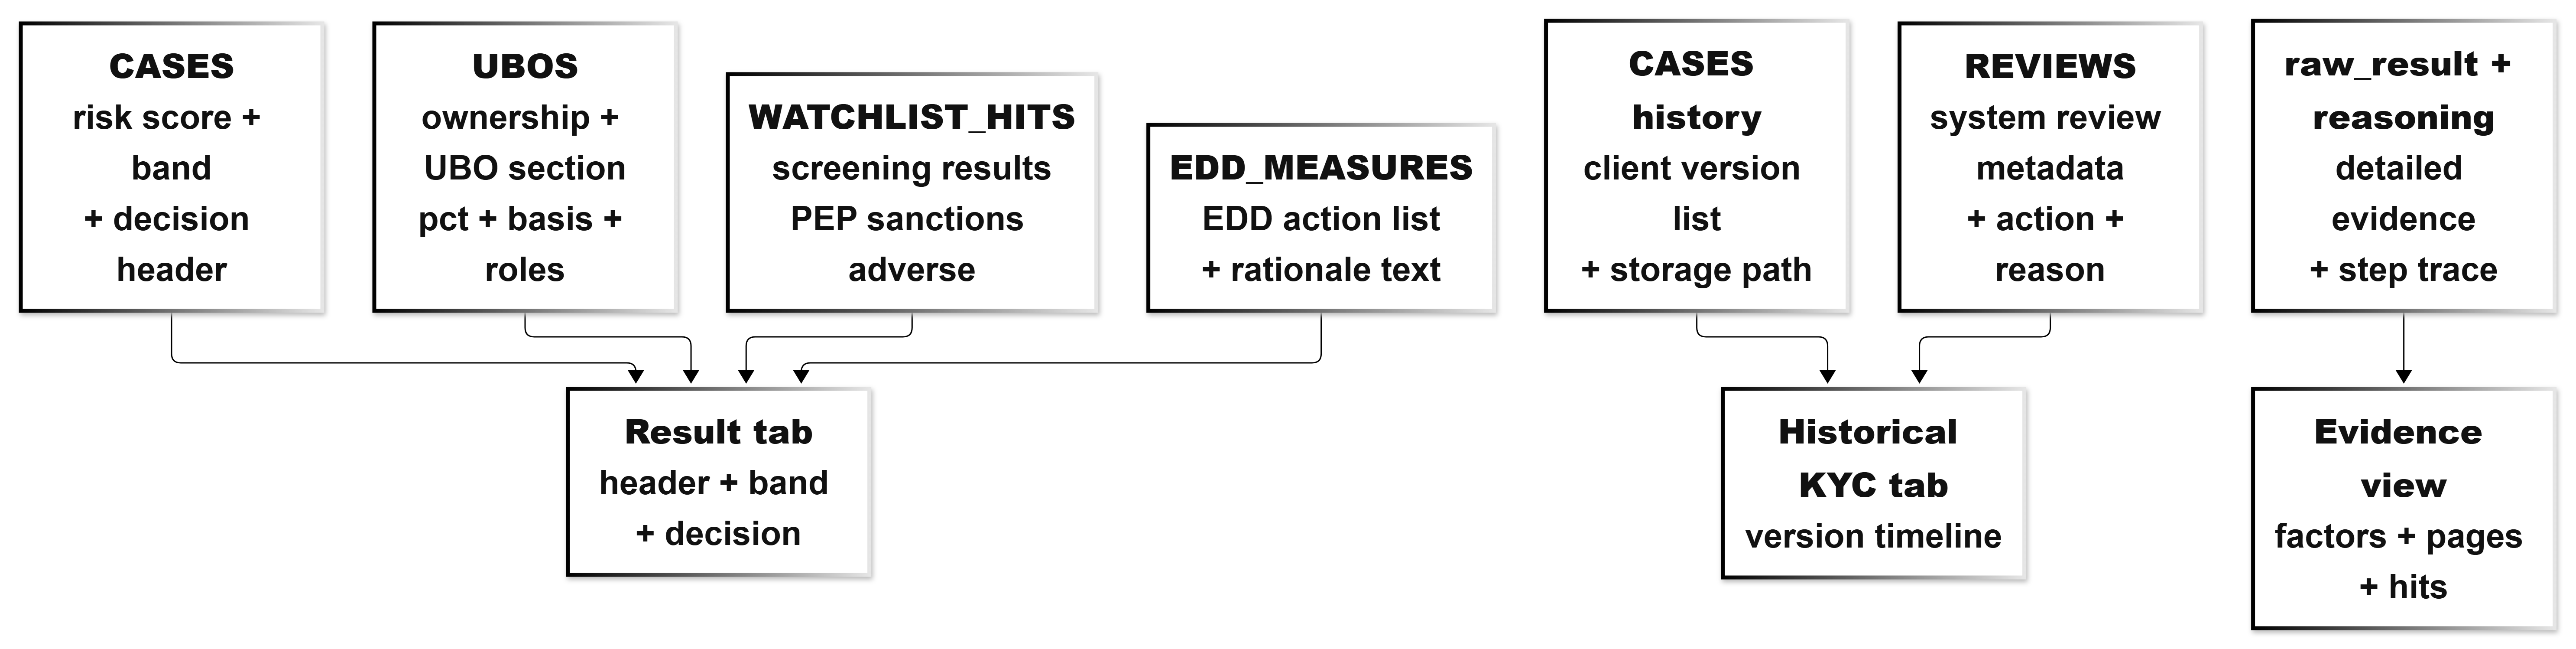
\includegraphics[width=\textwidth,height=0.85\textheight,keepaspectratio]{../diagrams/fraud_detection/05_flowchart_10-5-data-flow-from-tables-to-ui.png}
\caption{Data Flow from Tables to UI}
\label{fig:ch05_hni_onboarding-05-flowchart-10-5-data-flow-from-tables-to-ui}
\end{figure}

\subsection{Modeling Principles}

\speaker{Candidate}{I would follow these principles:}

\begin{enumerate}[leftmargin=\speakwid]
\item A case is one assessment version.
\item Historical assessments are append-only versions rather than overwritten results.
\item Deterministic derived outputs should be queryable in relational tables.
\item Full extraction evidence should be retained in \texttt{raw\_result} and analysis files until richer relational tables are implemented.
\item UBO and screening rows should be replaced atomically when a case is saved.
\item Every result should preserve source page or URL evidence where available.
\item A system-generated review must not be confused with human approval.
\end{enumerate}
\speaker{Interviewer}{Why not immediately normalize parties and ownership edges?}

\speaker{Candidate}{I would normalize them because ownership queries and audit reports become easier. In my design raw extracted structure stays in JSON and only the derived objects are stored relationally, and I would describe that boundary exactly rather than claim scope outside it.}

\speaker{Candidate}{With the data model fixed, may I walk through the analyst experience --- Document Upload, Name Search, and Historical KYC views?}

\medskip\hrule\medskip
\section{Product Screens and Reader Walkthrough}
\label{sec:ch05_hni_onboarding-11-product-screens-and-reader-walkthrough}

The product has three main user-facing workflows: Document Upload, Name Search, and Historical KYC.

\subsection{Document Upload View}

The Document Upload screen lets the analyst select one or more KYC PDFs, enter a client name, and start the assessment. The user-facing wording explains that the system accepts KYC forms, trust deeds, ownership charts, and identity documents.

The button initiates \texttt{POST /cases} with \texttt{case\_type=documents}. The response is queued while background processing continues.


\begin{figure}[htbp]
\centering
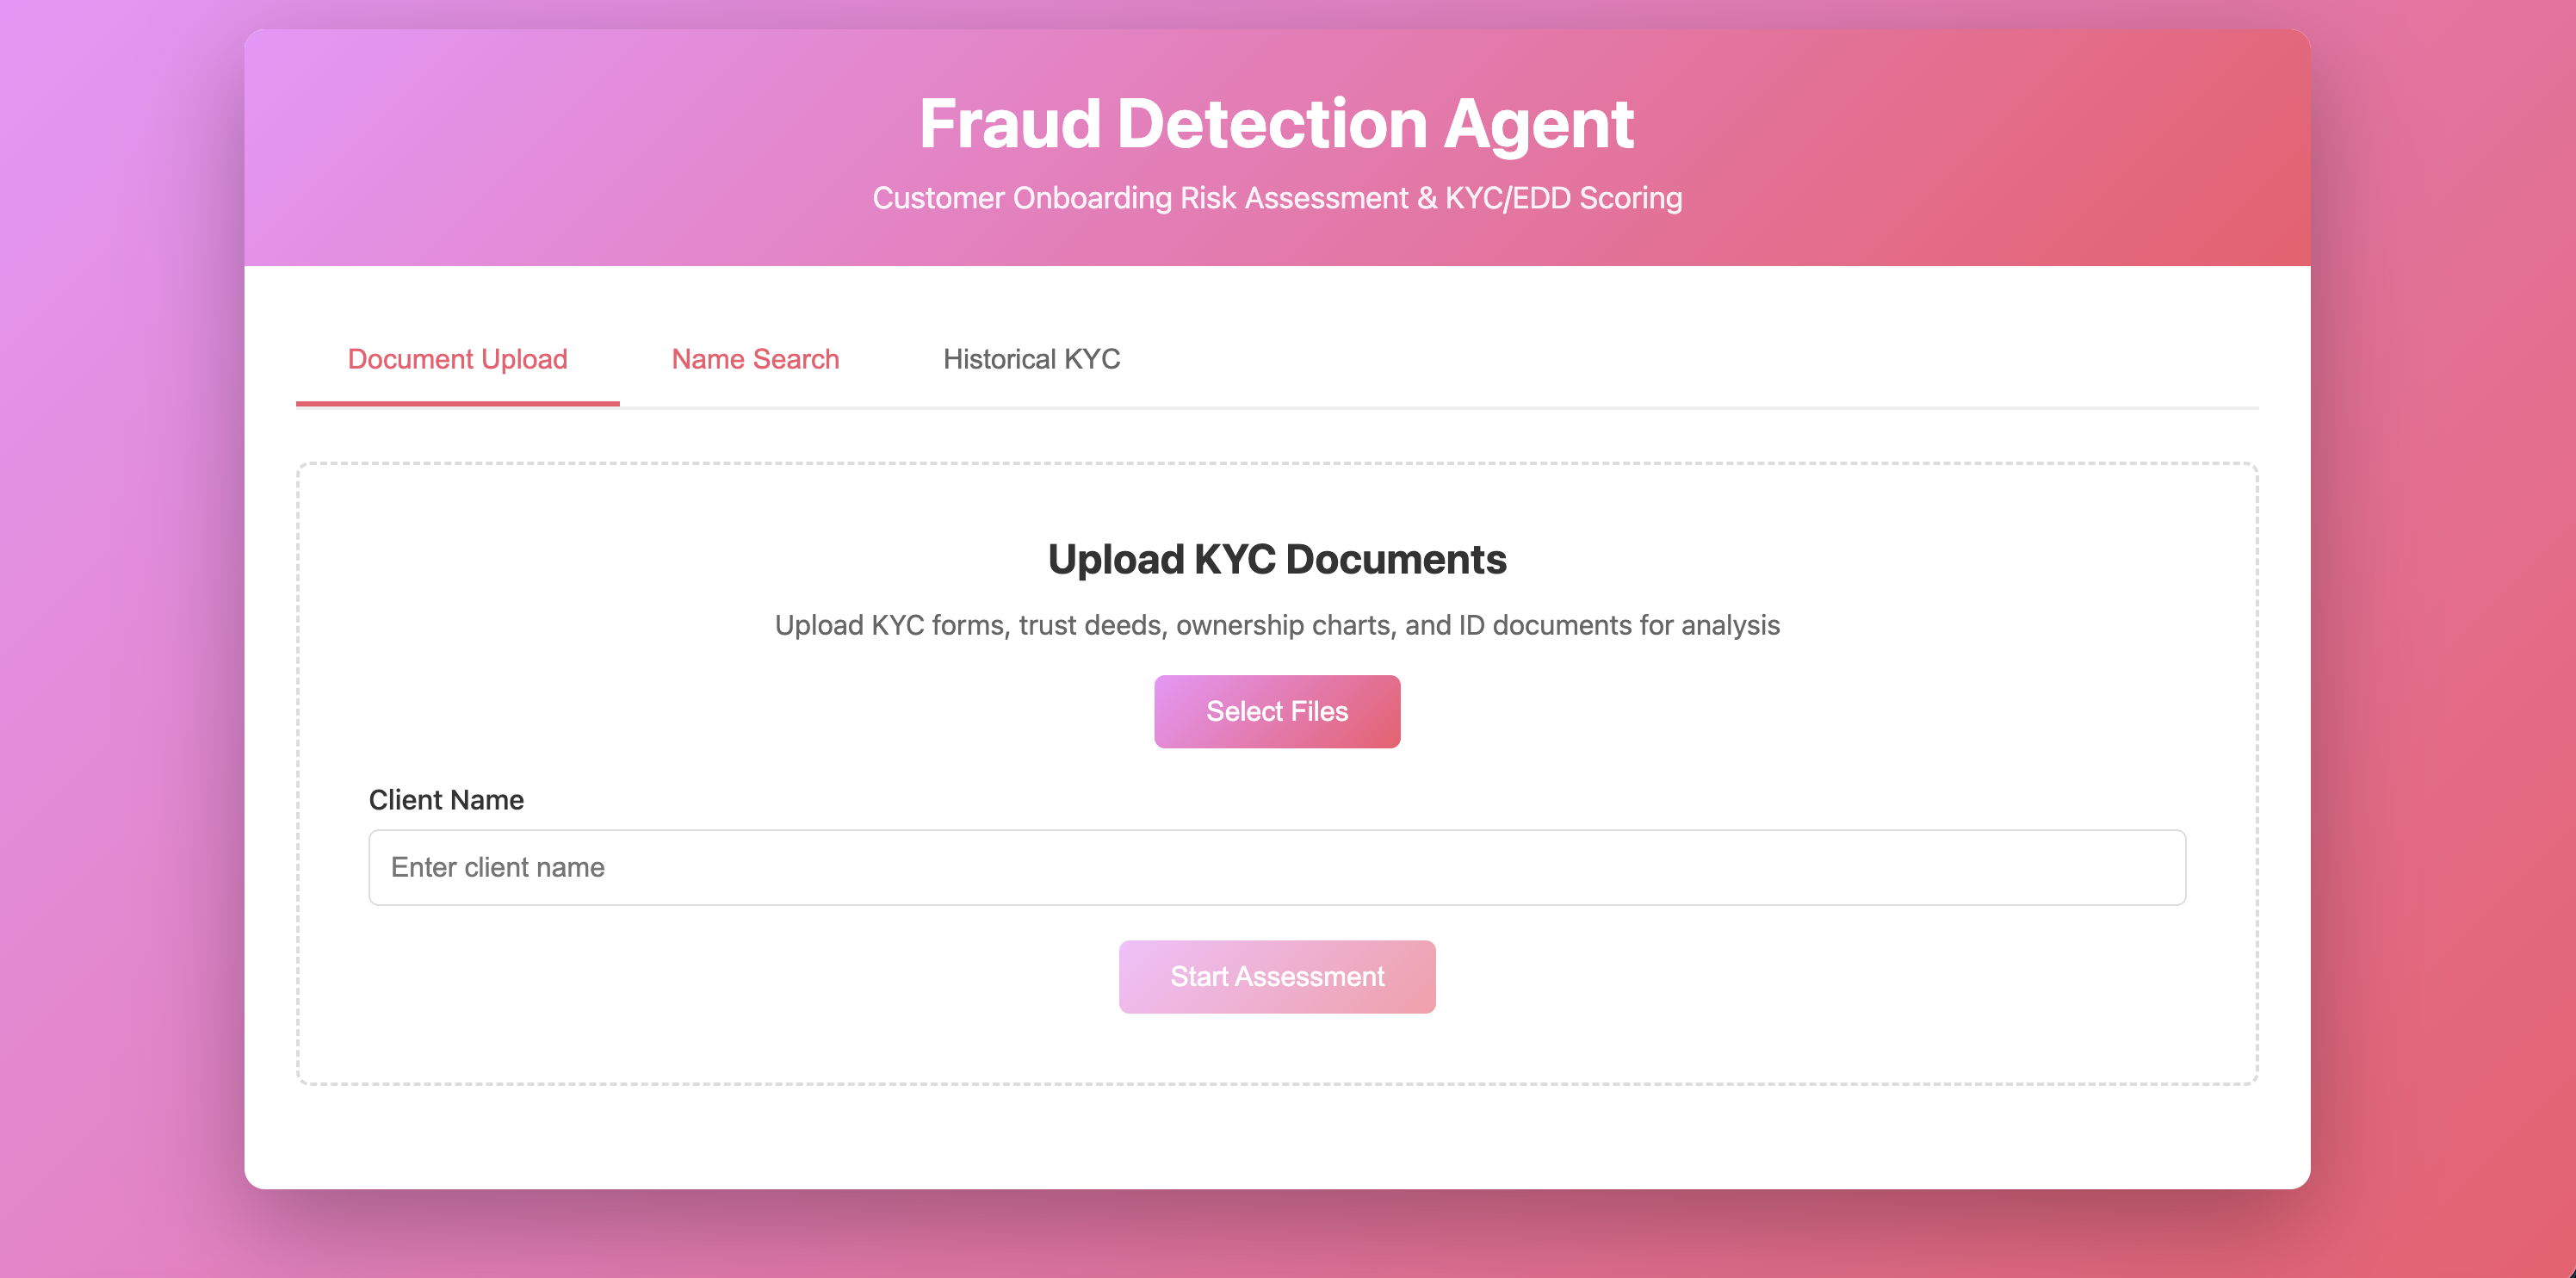
\includegraphics[width=\textwidth,height=0.85\textheight,keepaspectratio]{../diagrams/fraud_detection/screen_11_1_upload.png}
\caption{Document upload view: select KYC PDFs, enter a client name, and start the assessment.}
\label{fig:ch05_hni_onboarding-screen-11-1-upload}
\end{figure}

\subsection{Name Search View}

The Name Search screen lets the analyst enter a client name and optionally provide approximate age and location. It starts an OSINT search without requiring documents.

The HTTP path primarily passes the client name to the API. Richer seed fields are available in development interfaces, so the production UI is narrower than the broader internal \texttt{SubjectSeed} model.


\begin{figure}[htbp]
\centering
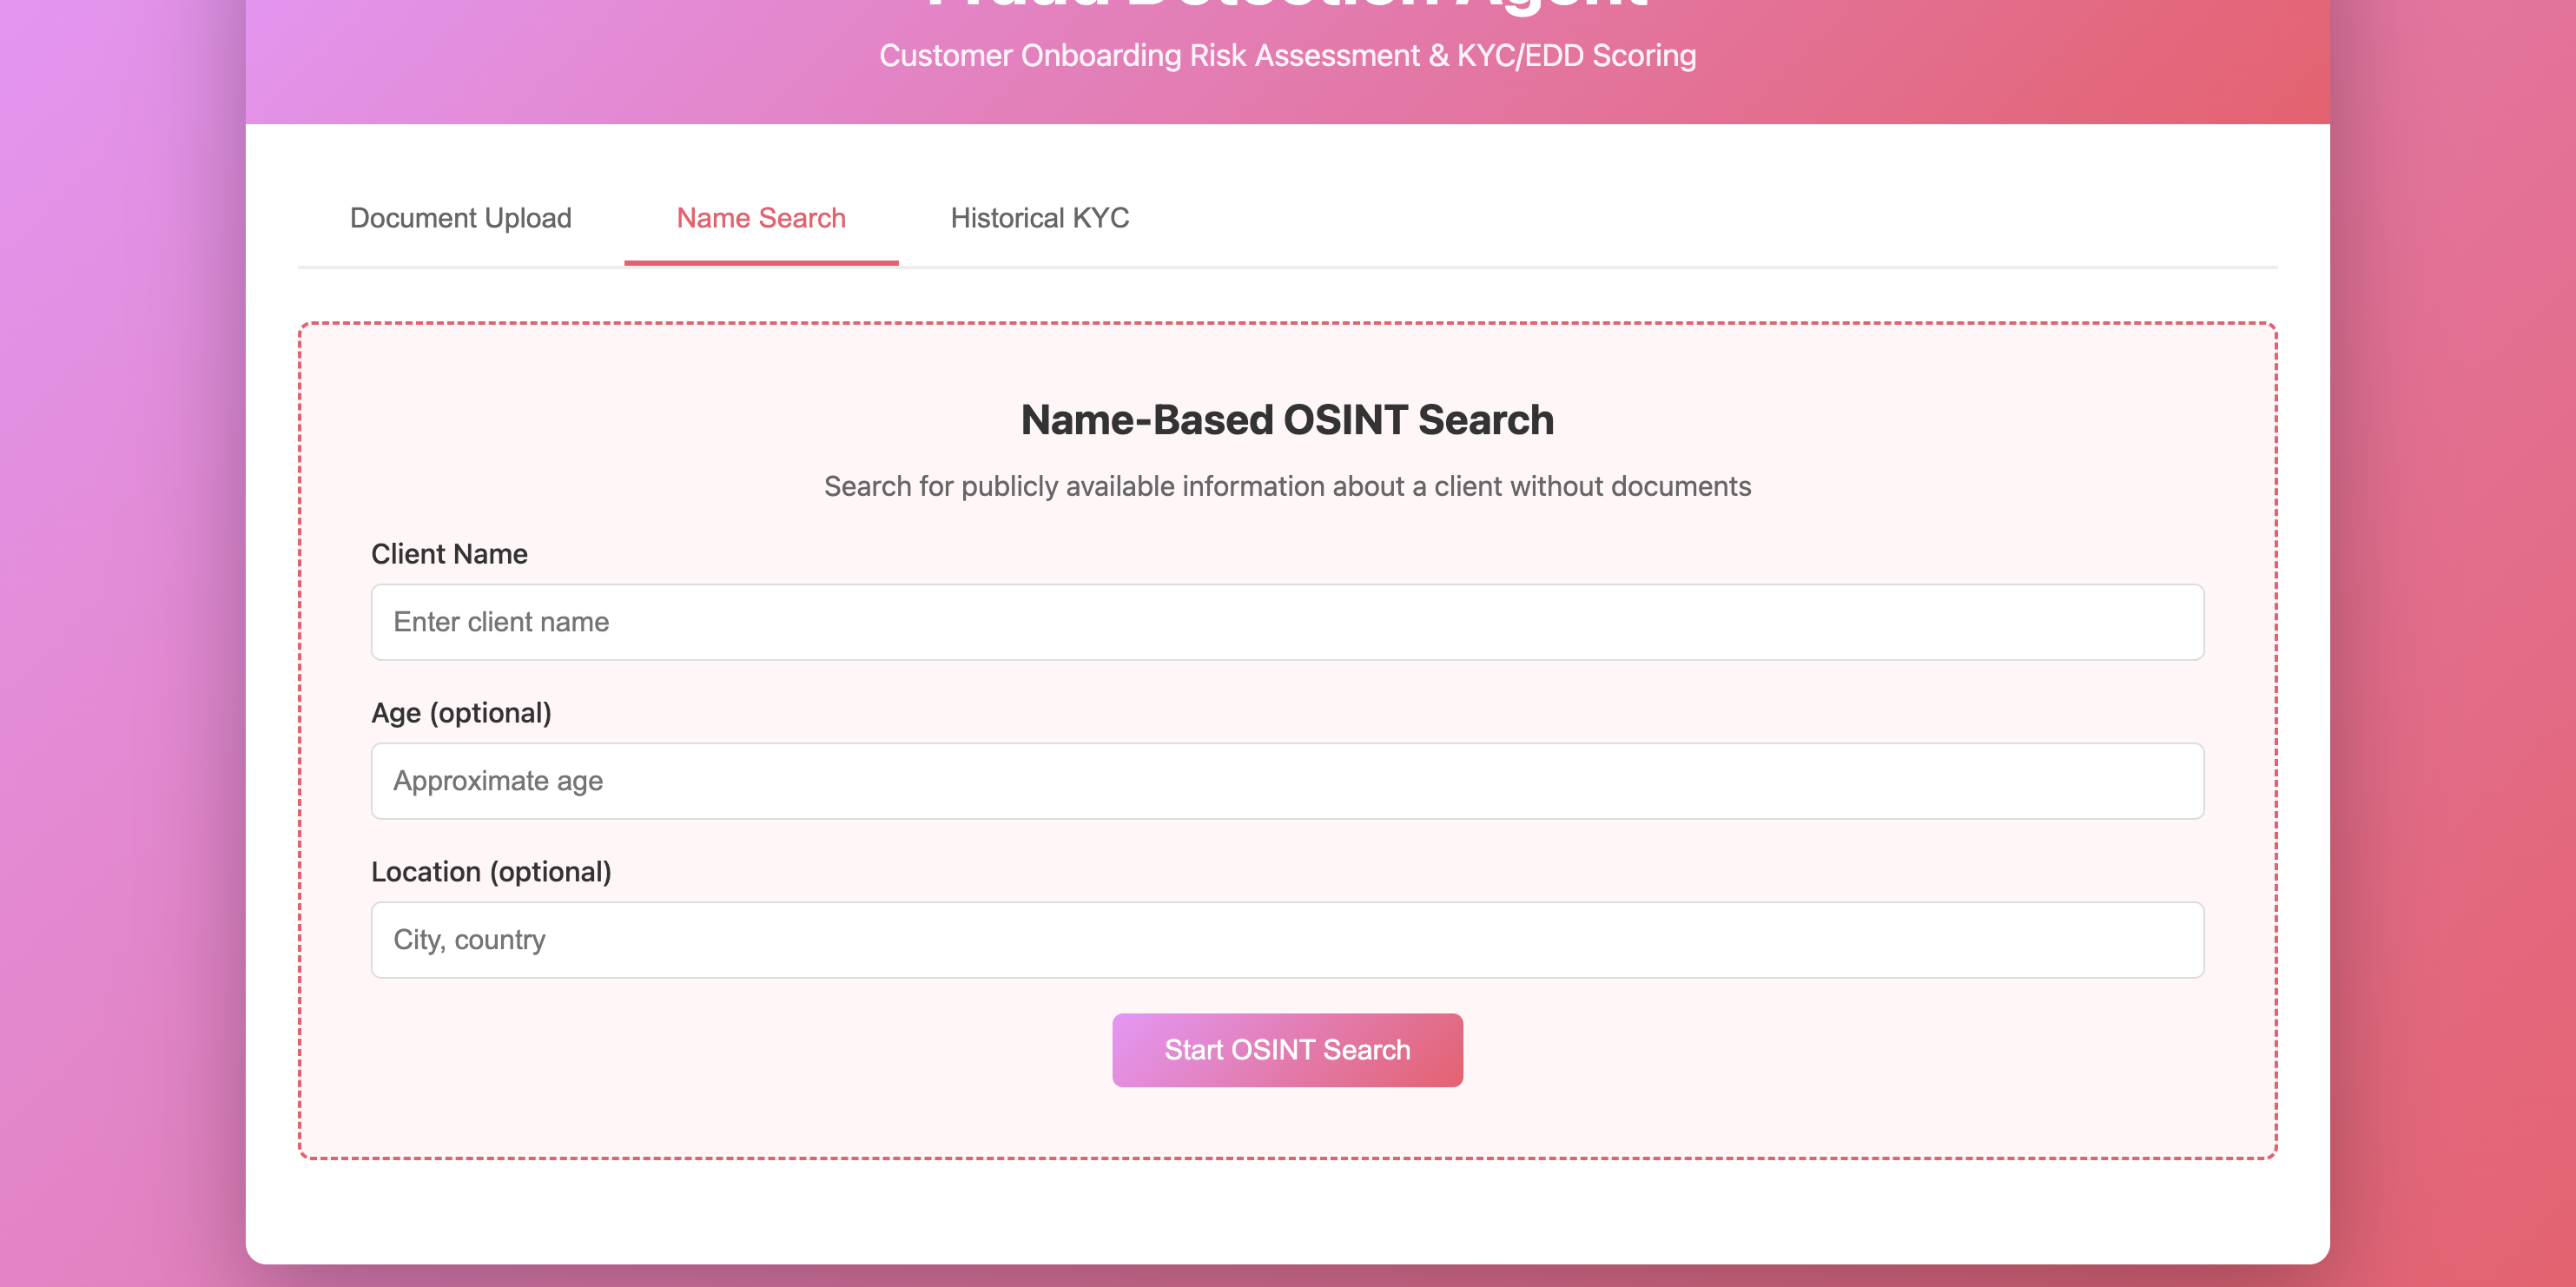
\includegraphics[width=\textwidth,height=0.85\textheight,keepaspectratio]{../diagrams/fraud_detection/screen_11_2_name_search.png}
\caption{Name search view: client name with optional age and location for a document-free OSINT search.}
\label{fig:ch05_hni_onboarding-screen-11-2-name-search}
\end{figure}

\subsection{Historical KYC View}

The Historical KYC screen allows an analyst to select a client and view previous assessments. Each history card can show:

\begin{itemize}[leftmargin=\speakwid]
\item Analysis type.
\item Version.
\item Date and time.
\item Processing status.
\item Risk score.
\item Risk band.
\item Recommended decision.
\end{itemize}
For example, a historical result may display a score of 59/100, a HIGH band, and an \texttt{ESCALATE\_MLRO} recommendation. Historical records are useful for periodic review, customer refresh, and comparing changes over time.


\begin{figure}[htbp]
\centering
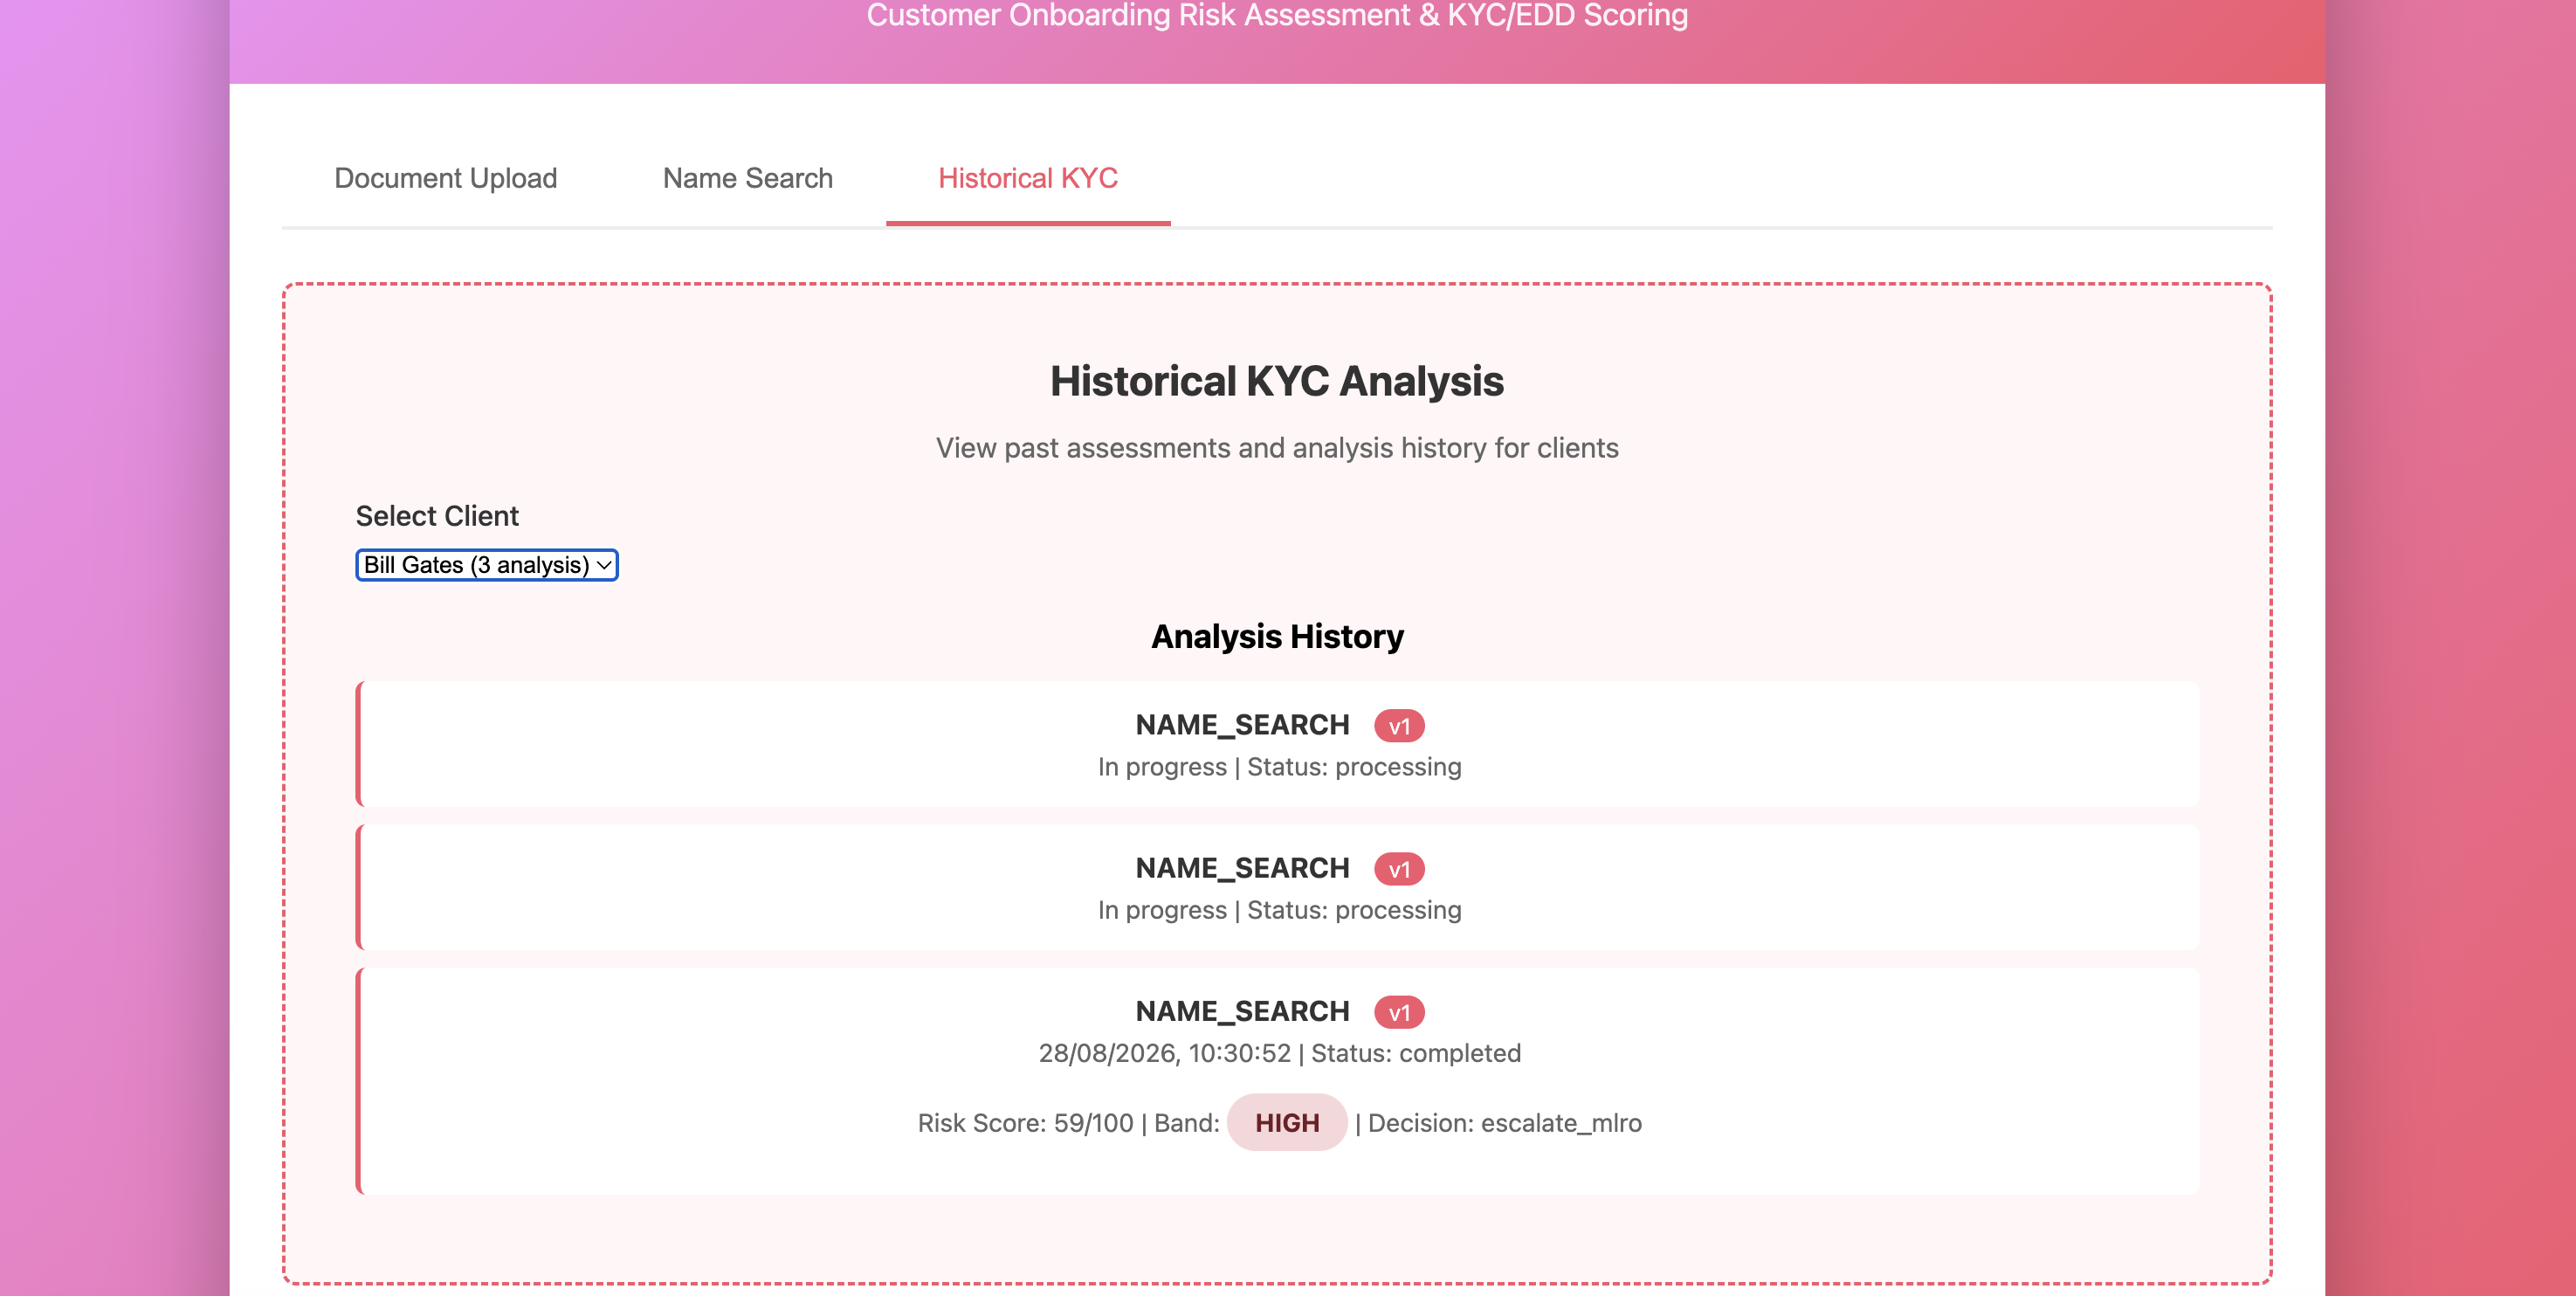
\includegraphics[width=\textwidth,height=0.85\textheight,keepaspectratio]{../diagrams/fraud_detection/screen_11_3_historical_kyc.png}
\caption{Historical KYC view: past assessments with analysis type, version, status, risk score, and decision.}
\label{fig:ch05_hni_onboarding-screen-11-3-historical-kyc}
\end{figure}

\subsection{Result Interpretation}

A useful product screen should distinguish:

\begin{itemize}[leftmargin=\speakwid]
\item Confirmed or curated screening hits.
\item Web-derived findings.
\item Missing information.
\item Hard stops.
\item EDD recommendations.
\item System-generated outputs awaiting human compliance review.
\end{itemize}
This distinction prevents users from treating a public-web signal as equivalent to a confirmed sanctions match.

\speaker{Interviewer}{The UI flow is clear. How will you evaluate extraction, UBO accuracy, sanctions/PEP screening, and risk scoring?}

\medskip\hrule\medskip
\section{Evaluation Framework}
\label{sec:ch05_hni_onboarding-12-evaluation-framework}

\speaker{Interviewer}{Now explain how you would evaluate this system. I want more than a single accuracy number.}

\speaker{Candidate}{I would evaluate it layer by layer.}

\subsection{Document Extraction Evaluation}

\begin{itemize}[leftmargin=\speakwid]
\item Party extraction precision and recall.
\item Party-type classification accuracy.
\item Ownership-edge precision and recall.
\item Relationship-role accuracy.
\item Applicant identification accuracy.
\item Source-of-wealth extraction accuracy.
\item Identity-document extraction accuracy.
\item Page-reference correctness.
\end{itemize}
\subsection{OSINT Evaluation}

\begin{itemize}[leftmargin=\speakwid]
\item Entity-disambiguation accuracy.
\item Evidence deduplication quality.
\item Adverse-media precision and recall.
\item PEP-indicator precision and recall.
\item Relationship extraction precision.
\item Source-of-wealth signal quality.
\item False-positive rate from common names.
\item Proportion of conclusions supported by retained URLs.
\end{itemize}
\subsection{Deterministic Engine Evaluation}

\begin{itemize}[leftmargin=\speakwid]
\item Effective-ownership correctness against manually calculated examples.
\item Control-based UBO correctness.
\item Cycle detection correctness.
\item Layering-depth correctness.
\item Watchlist token-match correctness.
\item Jurisdiction-tier correctness.
\item Score reproducibility.
\item Hard-stop correctness.
\item Decision and EDD-trigger correctness.
\end{itemize}
\subsection{Narrative Evaluation}

\begin{itemize}[leftmargin=\speakwid]
\item EDD rationale completeness.
\item Agreement with authoritative scorecard values.
\item Unsupported-claim rate.
\item Quality of recommended EDD measures.
\item Correct identification of missing information.
\item Separation of evidence from assumptions.
\end{itemize}
\subsection{Workflow Evaluation}

\begin{itemize}[leftmargin=\speakwid]
\item Successful document-case completion rate.
\item Successful name-search completion rate.
\item Median and p95 processing latency.
\item OSINT failure and fail-soft rates.
\item Percentage of cases with historical version records.
\item Database commit failure rate.
\item Percentage of results requiring manual correction.
\end{itemize}
\speaker{Interviewer}{How would you create a test dataset?}

\speaker{Candidate}{I would create a labelled dataset with:}

\begin{itemize}[leftmargin=\speakwid]
\item Simple individual cases.
\item Multi-layer holding-company structures.
\item Trusts and foundations.
\item Nominee and bearer-share mentions.
\item Missing ownership percentages.
\item Circular ownership.
\item Sanctions and PEP matches.
\item Common-name OSINT collisions.
\item High-risk and prohibited jurisdictions.
\item Missing source-of-wealth or identity evidence.
\item Empty or inaccessible public-search results.
\end{itemize}
\speakcont{Each case would have expected parties, edges, UBOs, screening hits, score factors, hard stops, band, decision, and EDD actions.}

\medskip\hrule\medskip
\section{Edge Cases and Failure Scenarios}
\label{sec:ch05_hni_onboarding-13-edge-cases-and-failure-scenarios}

\speaker{Interviewer}{Good. Now let us stress test the design.}

\subsection{Case 1: Missing Client Name}

\speaker{Interviewer}{What happens if the user uploads files without a client name?}

\speaker{Candidate}{The API rejects the request because \texttt{client\_name} is mandatory. The system should not start a case without a stable customer identity.}

\subsection{Case 2: Unknown Case Type}

\speaker{Interviewer}{What happens if the user sends an invalid case type?}

\speaker{Candidate}{My design must validate \texttt{case\_type} with an enum before accepting the request; returning a case ID without scheduling a task would leave the case rowless and effectively stuck.}

\subsection{Case 3: Document Case Without Files}

\speaker{Interviewer}{What if the user selects Document Upload but submits no PDFs?}

\speaker{Candidate}{My design rejects the request explicitly with a clear ``at least one PDF is required'' validation error when no PDFs arrive, rather than accepting a document case without scheduling its task.}

\subsection{Case 4: Scanned PDF}

\speaker{Interviewer}{What if the KYC document is image-only?}

\speaker{Candidate}{My design's page loader relies on text extraction and provides no OCR. It fails the document case rather than generating an empty low-risk result. OCR sits outside the design scope.}

\subsection{Case 5: No Public Evidence}

\speaker{Interviewer}{What if the name search finds nothing?}

\speaker{Candidate}{The profile becomes near-empty, but that does not mean the client is low risk. The result should state that public evidence is limited and should recommend obtaining documentary KYC evidence where appropriate.}

\subsection{Case 6: Common Name}

\speaker{Interviewer}{The name is ``John Smith,'' and search results belong to several people. What happens?}

\speaker{Candidate}{The profile reports low disambiguation confidence. The system should avoid presenting unrelated adverse findings as confirmed facts. The analyst should provide more context such as location, age, nationality, employer, or known companies.}

\subsection{Case 7: Sanctions Match}

\speaker{Interviewer}{What if a party matches a sanctions reference entry at 0.92 similarity?}

\speaker{Candidate}{The match is retained because it exceeds the 0.85 threshold. Sanctions are a hard-stop factor, so the case becomes PROHIBITED and the decision maps to DECLINE, subject to authorized human review and applicable policy.}

\subsection{Case 8: Prohibited Jurisdiction}

\speaker{Interviewer}{What if the applicant is incorporated in a prohibited jurisdiction?}

\speaker{Candidate}{The geography engine creates a prohibited-tier hit, the scorecard sets a hard-stop reason, and the decision becomes DECLINE.}

\subsection{Case 9: High-Risk Jurisdiction Only}

\speaker{Interviewer}{What if the jurisdiction is high risk but not prohibited?}

\speaker{Candidate}{The high-risk-geography factor activates with medium severity. It can trigger EDD and contribute to a MEDIUM or HIGH score, but it is not automatically a hard stop.}

\subsection{Case 10: Missing Ownership Percentage}

\speaker{Interviewer}{A trust deed identifies a trustee and protector but provides no percentage. What happens?}

\speaker{Candidate}{The system preserves the roles and can qualify control-based UBOs. It does not invent an ownership percentage. EDD may require additional ownership or control evidence.}

\subsection{Case 11: Circular Ownership}

\speaker{Interviewer}{What if Company A owns Company B and Company B owns Company A?}

\speaker{Candidate}{DFS detects the cycle, avoids infinite recursion, records circular ownership, and activates complex-structure or opacity-related scoring factors.}

\subsection{Case 12: Single Web Article}

\speaker{Interviewer}{One article alleges fraud. Should that automatically create a high adverse-media score?}

\speaker{Candidate}{No. A single web hit is discounted and capped at medium. The result should preserve the URL and recommend analyst verification. Multiple consistent high-severity web findings can increase severity, but curated evidence should remain more trusted.}

\subsection{Case 13: OSINT Provider Failure}

\speaker{Interviewer}{What if DuckDuckGo or Google is unavailable?}

\speaker{Candidate}{The name-search flow should complete with empty or partial evidence, clearly exposing the gap. It should not treat missing search results as evidence of clean history.}

\subsection{Case 14: Database Commit Failure}

\speaker{Interviewer}{What happens if analysis files are saved but the Postgres commit fails?}

\speaker{Candidate}{My design's outer error handling may swallow the database error, leaving files but no usable case row. This is a known gap. I would change the design to record durable job status, retry the transaction, and surface a failed or persistence-pending status.}

\subsection{Case 15: Concurrent Historical Assessments}

\speaker{Interviewer}{Two cases for the same client finish at the same time. Can both become version 2?}

\speaker{Candidate}{My design provides no guard for that race. I would enforce client-scoped sequencing with a database lock or unique constraint.}

\subsection{Case 16: Analyst Override}

\speaker{Interviewer}{Can an analyst correct a false positive or approve the case through the API?}

\speaker{Candidate}{No. My design provides no human review, correction, rerun, or question endpoints. Only a system-generated review row is written automatically. I would note those controls as required enhancements for a production compliance workflow.}

\subsection{Case 17: Low-Confidence Extraction Retry}

\speaker{Interviewer}{The extractor returns valid JSON but half the party types are wrong. Do you fail the case?}

\speaker{Candidate}{No. The correctness gate reports percent correct below 0.50, lists failures such as invalid party type or ungrounded name, appends them to the prompt, and reinvokes once. If the second attempt still scores low, the pipeline keeps the best attempt fail-soft and continues to UBO, screening, and scoring, so a weak extraction degrades EDD confidence rather than silently blocking onboarding.}

\subsection{Case 18: Uncited Adverse Claim in Name Search}

\speaker{Interviewer}{The profile alleges fraud but the URL was never in the collected evidence. How is that handled?}

\speaker{Candidate}{The suggestion gate flags \texttt{uncited\_adverse}, treats confidence as below threshold, and reinvokes with the failure listed so the model either grounds the claim or drops it. For the MLRO this prevents an invented link from becoming a web-derived watchlist hit and keeps the credibility discount --- single web source capped at medium --- honest.}

\speaker{Interviewer}{Edge cases covered. How would you deploy and operate this KYC platform reliably?}

\medskip\hrule\medskip
\section{Deployment and Operations}
\label{sec:ch05_hni_onboarding-14-deployment-and-operations}

\speaker{Interviewer}{How would you deploy this system?}

\speaker{Candidate}{I would start with one FastAPI service, one Postgres database, S3 or ADLS object storage, and the web UI served by the API. Two Streamlit development UIs exist outside the production Docker path.}

\subsection{Current Operational Shape}

\begin{itemize}[leftmargin=\speakwid]
\item One FastAPI process.
\item In-process background tasks.
\item Postgres as the source of truth for stored results.
\item S3 or ADLS upload and analysis prefixes.
\item In-memory page index during document processing.
\item External LLM gateway.
\item Internet access for name-search OSINT.
\item One replica for operational simplicity.
\end{itemize}
\subsection{Why Single Replica Matters}

\speaker{Candidate}{The assessment workflow is case-centric and sequential, so a single service keeps the first deployment simple. Because documents and analysis artifacts live in shared object storage with durable URIs, additional replicas and workers can locate the same files.}

\speaker{Interviewer}{What would you change before scaling horizontally?}

\speaker{Candidate}{I would:}

\begin{enumerate}[leftmargin=\speakwid]
\item Add a durable task queue.
\item Make processing idempotent.
\item Add job leasing and recovery.
\item Persist page chunks or use a shared vector index.
\item Add authentication, authorization, and tenant isolation.
\end{enumerate}
\subsection{Monitoring Needs}

\begin{itemize}[leftmargin=\speakwid]
\item API health and latency.
\item Queued, completed, failed, and rowless cases.
\item Background-task duration.
\item LLM calls, token usage, and errors.
\item OSINT provider availability.
\item Page extraction failures.
\item UBO and screening match counts.
\item Hard-stop counts.
\item EDD-trigger rates.
\item Database commit failures.
\item Storage errors.
\item Historical-version conflicts.
\end{itemize}

\speaker{Interviewer}{Operations are clear. What gaps remain before this EDD workflow is production-hardened?}

\medskip\hrule\medskip
\section{Current Gaps and Enhancement Roadmap}
\label{sec:ch05_hni_onboarding-15-current-gaps-and-enhancement-roadmap}

\speaker{Interviewer}{What are the most important gaps in your design?}

\speaker{Candidate}{I would separate them into correctness, reliability, security, and product gaps.}

\subsection{Current Gaps}

\begin{enumerate}[leftmargin=\speakwid]
\item No OCR support for scanned PDFs.
\item The API does not write a queued processing row before the background task.
\item Database commit errors can leave a completed analysis rowless.
\item Invalid case types or missing document files may create a case ID without scheduling work.
\item Parties, page chunks, documents, and ownership edges are declared but not populated relationally.
\item Reference watchlists are sample or configurable fixtures rather than complete commercial feeds.
\item No human review, correction, rerun, or HTTP Q\&A endpoints.
\item Object-storage lifecycle and versioning need hardening before aggressive horizontal scaling.
\item Name-search disambiguation can be weak for common names.
\item Version assignment needs stronger concurrency control.
\item Authentication, RBAC, tenant isolation, and privacy controls need production hardening.
\end{enumerate}

\speaker{Candidate}{May I add one clarification before the short-term list, so the gap table does not mislead? The row about parties, page chunks, documents, and ownership edges being unpopulated needs a precise reading.}

\speaker{Interviewer}{How should a reader interpret it?}

\speaker{Candidate}{Those four tables are written by \texttt{persist\_case\_graph()} and EDD category and severity are set by \texttt{classify\_edd\_measure()}, verified by offline validation tests. Remaining gaps are unresolved configuration keys, swallowed commit errors, missing human review and rerun endpoints, sample-only reference lists, no OCR, and concurrency hardening around version assignment --- so the roadmap below still applies, just without re-normalizing tables that already persist.}
\subsection{Short-Term Enhancements}

\begin{itemize}[leftmargin=\speakwid]
\item Validate \texttt{case\_type} and file requirements at the API boundary.
\item Insert a durable queued case row before scheduling work.
\item Improve persistence error handling and retries.
\item Add explicit OCR or a clear scanned-document workflow.
\item Add OSINT source-quality and disambiguation indicators.
\item Add detailed processing phases.
\end{itemize}
\subsection{Production Enhancements}

\begin{itemize}[leftmargin=\speakwid]
\item Move storage to S3 or equivalent.
\item Add durable queue workers.
\item Add authentication, RBAC, and MLRO approval workflows.
\item Add real sanctions, PEP, and adverse-media providers.
\item Normalize parties and ownership edges.
\item Add immutable audit events.
\item Add database constraints for versioning and idempotency.
\end{itemize}
\subsection{Advanced Enhancements}

\begin{itemize}[leftmargin=\speakwid]
\item Entity resolution using identity attributes and aliases.
\item Graph database or graph-query layer for complex ownership structures.
\item Periodic KYC refresh and change detection.
\item Transaction-monitoring integration.
\item Portfolio-level customer-risk analytics.
\item Human-feedback loops for false-positive reduction.
\item Policy retrieval for jurisdiction-specific EDD requirements.
\end{itemize}

\speaker{Candidate}{With the roadmap agreed, I am ready for your final questions on ownership, risk, and EDD trade-offs.}

\medskip\hrule\medskip
\section{Final Interview Discussion}
\label{sec:ch05_hni_onboarding-16-final-interview-discussion}

\speaker{Interviewer}{Let me ask a few final questions. Why is this an agentic AI system rather than a normal rules engine?}

\speaker{Candidate}{The system uses language models to extract parties and relationships from unstructured KYC documents and to synthesize a public profile from multiple evidence snippets. Those tasks require language understanding across varied documents and sources. But the system does not hand final authority to the model. It combines agent-like evidence processing with deterministic compliance logic.}

\speaker{Interviewer}{Where would you explicitly avoid using an LLM?}

\speaker{Candidate}{I would avoid using it for effective-ownership math, watchlist threshold decisions, risk weights, severity multipliers, hard stops, risk bands, and final decision mapping. Those must be deterministic and testable.}

\speaker{Interviewer}{Why have both document upload and name search?}

\speaker{Candidate}{Document upload provides stronger private evidence for onboarding, while name search provides a preliminary public-information view when documents are unavailable or before they arrive. They serve different operational moments but can share the same risk engine.}

\speaker{Interviewer}{What is the most dangerous false positive in this system?}

\speaker{Candidate}{A wrongly attributed sanctions or adverse-media finding caused by name collision. That is why identity context, source provenance, disambiguation confidence, and human review are essential.}

\speaker{Interviewer}{What is the most dangerous false negative?}

\speaker{Candidate}{Treating missing evidence as clean evidence, for example, returning low risk because OSINT found nothing, or because a scanned PDF produced no extractable text. The system must distinguish ``no risk found'' from ``insufficient evidence.''}

\speaker{Interviewer}{Summarize the complete design in one paragraph.}

\speaker{Candidate}{I would build a versioned KYC onboarding-risk platform with two entry points: document upload and name-based OSINT search. FastAPI accepts the request quickly and runs the selected workflow in the background. Document agents extract parties, ownership, source-of-wealth, identity, and applicant metadata; the name workflow collects public evidence and synthesizes a profile. Both flows then use deterministic Python to resolve UBOs, screen names and jurisdictions, calculate an eleven-factor risk score, enforce sanctions and prohibited-jurisdiction hard stops, map the result to a risk band and decision, and trigger EDD where needed. An LLM writes a grounded EDD rationale from compact scorecard JSON, while Postgres and analysis files preserve versions, derived results, and evidence for historical KYC review.}

\speaker{Interviewer}{Good. You clarified the business problem first, separated public evidence from documentary evidence, kept critical decisions deterministic, and worked through the scope honestly.}

\speaker{Candidate}{Thank you.}

\section*{Source Code}

The complete implementation for the HNI Customer Onboarding Agent is available in the accompanying GitHub repository:

\begin{center}
\url{https://github.com/GSaiDheeraj/Finance-and-Banking-AI-Usecases/tree/main/HNI_Customer_Onboard_KYC_Agent}
\end{center}
